\documentclass[handout]{beamer}
\usepackage{pgfpages}
\pgfpagesuselayout{4 on 1}[a4paper,border shrink=5mm, landscape] % possibly: 4 on 1, add "landscape" to options
\useinnertheme{rectangles}
%\usepackage{paralist} % for compactitem    conflicts with enumerate!!!!!!!
\usepackage{graphicx}
\usetheme{Warsaw}

\usepackage{xcolor}
\definecolor{light-gray}{gray}{0.9}
\definecolor{dark-red}{HTML}{990000}
\setbeamertemplate{headline}{}
\setbeamercolor{frametitle}{fg=dark-red,bg=light-gray}
\setbeamercolor{author in head/foot}{bg=dark-red}

\setbeamercolor{normal text}{fg=black,bg=white}
\setbeamercolor{alerted text}{fg=green!60!black}

\setbeamercolor{structure}{fg=dark-red}

\setbeamercolor{background canvas}{parent=normal text}
\setbeamercolor{background}{parent=background canvas}

\setbeamercolor{palette primary}{fg=white,bg=white} % changed this
\setbeamercolor{palette secondary}{fg=black, bg=green!60!black} % changed this
\setbeamercolor{palette tertiary}{} %

\setbeamertemplate{itemize item}[triangle]
%\setbeamertemplate{itemize item}[square]    %%% for big square in itemize
\setbeamertemplate{itemize subitem}{\tiny\raise0.5ex\hbox{\rule{0.5em}{0.5em}}}
%\setbeamertemplate{itemize subitme}[circle]   %% circle in subitem

\setbeamertemplate{enumerate items}[square]

\setbeamertemplate{blocks}[rounded][shadow=false]
\setbeamercolor{block title}{fg=white, bg=dark-red}
\setbeamercolor{block body}{fg=black, bg=light-gray}

\setbeamertemplate{section in toc}{%
  {\color{dark-red}}~\inserttocsection}

\setbeamertemplate{subsection in toc}{%
  \hspace{1.2em}{\color{dark-red}\rule[0.3ex]{3pt}{3pt}}~\inserttocsubsection\par}


\setbeamertemplate{footline}
{
  \leavevmode%
  \hbox{%
  \begin{beamercolorbox}[wd=.35\paperwidth,ht=2.25ex,dp=1ex,center]{author in head/foot}%
    \usebeamerfont{author in head/foot}\insertauthor
  \end{beamercolorbox}%
  \begin{beamercolorbox}[wd=.3\paperwidth,ht=2.25ex,dp=1ex,center]{frametitle}%
    \usebeamerfont{title in head/foot}\insertsection
  \end{beamercolorbox}%
  \begin{beamercolorbox}[wd=.35\paperwidth,ht=2.25ex,dp=1ex,center]{author in head/foot}%
    \usebeamerfont{date in head/foot}
    \insertinstitute
   %%%%%%%%%%%%%% frame numbers %%%%%%%%%%%%%
   % \insertframenumber{} / \inserttotalframenumber\hspace*{2ex} 
   %%%%%%%%%%%%%%%%%%%%%%%%%%%%%%%%%%%%%%%%%%
  \end{beamercolorbox}}%
  \vskip0pt%
}

\setbeamertemplate{frametitle}
{
	\vspace{1.5ex}
    \nointerlineskip
    \begin{beamercolorbox}[rounded=true,left,wd=\paperwidth]{frametitle}
        \vbox{}
        \strut\insertframetitle\strut
    \end{beamercolorbox}
}
\setbeamertemplate{title page}
{
	\vspace*{10pt}
	\parbox{0.45\linewidth}{
		\hspace*{-100pt}
    	\begin{beamercolorbox}[rounded=true,right, wd=0.45\paperwidth, ht=0.6em, dp=0.1em]
    	{frametitle}
			\usebeamerfont{author}
        	\vbox{}
        	\hspace*{70pt}\hfill\strut\insertdate\strut\hspace*{5pt}
    	\end{beamercolorbox}
    }	
	\parbox{0.5\linewidth}{
		\hfill
		\vspace*{-30pt}
		\placelogotrue
		\hfill\insertlogo
		\placelogofalse
		\hspace*{-30pt}
	}\\
    \vfill
    \vspace*{160pt}
	\hspace*{-100pt}
	\begin{beamercolorbox}[rounded=true,right, wd=0.9\paperwidth]{frametitle}%
		\usebeamerfont{title}
        \vbox{}
        \hspace*{100pt}\hfill\strut\inserttitle\strut\hspace*{5pt}
    \end{beamercolorbox}%
    \\
    \hspace*{-100pt}
    \begin{beamercolorbox}[rounded=true,right, wd=0.9\paperwidth, ht=0.6em, dp=0.1em]
    {author in head/foot}%
		\usebeamerfont{author}
        \vbox{}
        \hspace*{100pt}\hfill\strut\insertauthor\strut\hspace*{5pt}
    \end{beamercolorbox}%

}

\setbeamertemplate{section page}
{


    \vfill
    \vspace*{160pt}
	\hspace*{-100pt}
	\begin{beamercolorbox}[rounded=true,right, wd=0.9\paperwidth]{frametitle}%
		\usebeamerfont{title}
        \vbox{}
        \hspace*{100pt}\hfill\strut\insertsection\strut\hspace*{5pt}
    \end{beamercolorbox}%
}

\setbeamertemplate{notes} 
{
}

\usepackage[utf8]{inputenc}
\usepackage[german]{babel}
\usepackage[T1]{fontenc}
\usepackage{amsmath}
\usepackage{amsfonts}
\usepackage{graphicx}
\usepackage{amssymb}
\usepackage{tikz, tkz-graph}
\usepackage{url}
\usetikzlibrary{graphs,fit}
\usetikzlibrary{positioning}   % for [right=of ..] etc.
\author{Ansgar Rössig, Arne Schmidt}
\title{Recurrent Neural Networks}
%\setbeamercovered{transparent} 
\setbeamertemplate{navigation symbols}{} 
\newif\ifplacelogo % create a new conditional
\logo{\ifplacelogo
\includegraphics[scale=0.4]{data/tu_logo.png}\fi} 
\institute{TU Berlin} 
\date{Feb 14$^\text{th}$, 2018} 
%\subject{} 
\begin{document}

{
\setbeamertemplate{footline}{} 
\begin{frame}
\titlepage
\end{frame}
}

\section*{Agenda}
\begin{frame}{Agenda}
\tableofcontents

\end{frame}

\section{Introduction}

\begin{frame}{Recurrent Neural Network Example}
\begin{overlayarea}{\textwidth}{7cm}
\only<1|handout:1>{
\begin{tikzpicture}[->, scale=0.6]
\tikzset{VertexStyle/.style = {shape=circle, inner sep = 2pt, minimum size = 16pt, draw}}
\tikzset{EdgeStyle/.style = {->, thick}}
  	\SetGraphUnit{1}
	\Vertex[x=0, y=0]{x}
	\Vertex[x=0, y=3]{h}
	\Vertex[x=0, y=6]{o}
	\Vertex[x=0, y=8]{L}
	\Vertex[x=0, y=10]{y}   	
  	\Edge[label=U](x)(h)
  	\Edge[label=V](h)(o)
  	\Loop[dir=WE, label={\qquad W}](h)
  	\Edge[](o)(L)
  	\Edge[](y)(L)
\tikzset{VertexStyle/.style = {}}
  	\Vertex[x=5, y=0, L={input value}]{xb}
	\Vertex[x=5, y=3, L={hidden neuron}]{hb}
	\Vertex[x=5, y=6, L={output neuron}]{ob}
	\Vertex[x=5, y=8, L={loss function}]{Lb}
	\Vertex[x=5, y=10, L={target value}]{yb}   
\end{tikzpicture}
}
\only<0|handout:2>{
% for notes
\begin{itemize}
\item RNNs are good to work with input sequences of unknown / variable length
\item parameters $U, V, W$ are shared accross multiple time steps
\item theoretically, the number of time steps is not bounded
\item in practice, a fixed number $\tau$ of time steps is used for all computations
\end{itemize}
}
\only<2|handout:3>{
\begin{tikzpicture}[->, scale=0.6]
\tikzset{VertexStyle/.style = {shape=circle, inner sep = 2pt, minimum size = 24pt, draw, font=\tiny}}
\tikzset{EdgeStyle/.style = {->, thick}}
  	\SetGraphUnit{1}
	\Vertex[x=-1, y=0]{x}
	\Vertex[x=-1, y=3]{h}
	\Vertex[x=-1, y=6]{o}
	\Vertex[x=-1, y=8]{L}
	\Vertex[x=-1, y=10]{y}   	
  	\Edge[label=U](x)(h)
  	\Edge[label=V](h)(o)
  	\Loop[dir=WE, label={\qquad W}](h)
  	\Edge[](o)(L)
  	\Edge[](y)(L)
  	
  	\Vertex[x=2, y=3, style={dotted}, L={$h^{(\ldots)}$}]{h0}
  	\Vertex[x=5, y=0, L={$x^{(t-1)}$}]{x1}
	\Vertex[x=5, y=3, L={$h^{(t-1)}$}]{h1}
	\Vertex[x=5, y=6, L={$o^{(t-1)}$}]{o1}
	\Vertex[x=5, y=8, L={$L^{(t-1)}$}]{L1}
	\Vertex[x=5, y=10, L={$y^{(t-1)}$}]{y1}   	
  	\Edge[label=U](x1)(h1)
  	\Edge[label=V](h1)(o1)
  	\Edge[label={\scriptsize W}](h0)(h1)
  	\Edge[](o1)(L1)
  	\Edge[](y1)(L1)
  	
  	\Vertex[x=8, y=0, L={$x^{(t)}$}]{x2}
	\Vertex[x=8, y=3, L={$h^{(t)}$}]{h2}
	\Vertex[x=8, y=6, L={$o^{(t)}$}]{o2}
	\Vertex[x=8, y=8, L={$L^{(t)}$}]{L2}
	\Vertex[x=8, y=10, L={$y^{(t)}$}]{y2}   	
  	\Edge[label=U](x2)(h2)
  	\Edge[label=V](h2)(o2)
  	\Edge[label={\scriptsize W}](h1)(h2)
  	\Edge[](o2)(L2)
  	\Edge[](y2)(L2)
  	
  	\Vertex[x=11, y=0, L={$x^{(t+1)}$}]{x3}
	\Vertex[x=11, y=3, L={$h^{(t+1)}$}]{h3}
	\Vertex[x=11, y=6, L={$o^{(t+1)}$}]{o3}
	\Vertex[x=11, y=8, L={$L^{(t+1)}$}]{L3}
	\Vertex[x=11, y=10, L={$y^{(t+1)}$}]{y3}   	
  	\Edge[label=U](x3)(h3)
  	\Edge[label=V](h3)(o3)
  	\Edge[label={\scriptsize W}](h2)(h3)
  	\Edge[](o3)(L3)
  	\Edge[](y3)(L3)
  	
  	\Vertex[x=14, y=3, style={dotted}, L={$h^{(\ldots)}$}]{h4}
  	\Edge[label={\scriptsize W}](h3)(h4)
  
\end{tikzpicture}
}
\end{overlayarea}
\end{frame}

\begin{frame}[beamer:0]{Notes}
\begin{itemize}
\item the unfolded computational graph shows how forward and back-propagation can be applied
\item it is assumed that the same parameters are relevant at all time steps
\end{itemize}
\end{frame}

\begin{frame}{Forward Propagation}
\parbox{0.25\textwidth}{
\begin{tikzpicture}[->, scale=0.6]
\tikzset{VertexStyle/.style = {shape=circle, inner sep = 0.3, minimum size = 16pt, draw}}
\tikzset{EdgeStyle/.style = {->, thick}}
  	\SetGraphUnit{1}
	\Vertex[x=0, y=0]{x}
	\Vertex[x=0, y=3]{h}
	\Vertex[x=0, y=6]{o}
	\Vertex[x=0, y=8]{L}
	\Vertex[x=0, y=10]{y}   	
  	\Edge[label=U](x)(h)
  	\Edge[label=V](h)(o)
  	\Loop[dir=WE, label={\qquad W}](h)
  	\Edge[](o)(L)
  	\Edge[](y)(L)
\end{tikzpicture}
}
\hfill
\parbox{0.65\textwidth}{
\begin{itemize}
\item start with initial state $h^{(0)}$
\item then for $t = 1, \ldots, \tau$:
\begin{align*}
a^{(t)} & = b + Wh^{(t-1)} + Ux^{(t)}\\
h^{(t)} & = \sigma(a^{(t)})\\
o^{(t)} & = c + Vh^{(t)}\\
\hat{y}^{(t)} & = \text{softmax}(o^{(t)})\\
\end{align*}
\end{itemize}
}
\end{frame}

\begin{frame}[beamer:0]{Notes}
\begin{itemize}
\item for forward propagation an initial state $h^{(0)}$ is fixed
\item then the inputs can be propagated forward through the unfolded computational graph as in the case of feedforward networks
\item this can be continued for arbitrarily many time steps, e.g. until the end of the input sequence is reached
\end{itemize}
\end{frame}

\begin{frame}{Back-propagation and loss function}
\parbox{0.25\textwidth}{
\begin{tikzpicture}[->, scale=0.6]
\tikzset{VertexStyle/.style = {shape=circle, inner sep = 0.3, minimum size = 16pt, draw}}
\tikzset{EdgeStyle/.style = {->, thick}}
  	\SetGraphUnit{1}
	\Vertex[x=0, y=0]{x}
	\Vertex[x=0, y=3]{h}
	\Vertex[x=0, y=6]{o}
	\Vertex[x=0, y=8]{L}
	\Vertex[x=0, y=10]{y}   	
  	\Edge[label=U](x)(h)
  	\Edge[label=V](h)(o)
  	\Loop[dir=WE, label={\qquad W}](h)
  	\Edge[](o)(L)
  	\Edge[](y)(L)
\end{tikzpicture}
}
\hfill
\parbox{0.65\textwidth}{
\begin{overlayarea}{0.65\textwidth}{8cm}
\only<1|handout:1>{
\begin{itemize}
\item let $L^{(t)}$ be the negative log-likelihood of $y^{(t)}$ given $x^{(1)}, \ldots, x^{(t)}$
\item sum the loss over all time steps \begin{align*}
& L(\{x^{(1)}, \ldots, x^{(\tau)}\}, \{y^{(1)}, \ldots, y^{(\tau)}\})\\
= & \sum_t L^{(t)}\\
= &- \sum_t \text{log } p_{model}(y^{(t)} \  | \ \{x^{(1)}, \ldots, x^{(t)}\})\\
= &- \sum_t \text{log } \hat{y}^{(t)}
\end{align*}
\item use back-propagation through time (BPTT)
\end{itemize}
}
\only<0|handout:2>{
\begin{itemize}
\item back-propagation through time (BPTT) is simply the normal back-propagation algorithm applied to the unfolded computational graph
\item BPTT is used to minimize the sum of the loss values at all time steps
\end{itemize}
}
\only<2-|handout:3>{
\begin{itemize}
\item parameters are shared across all time steps
\item therefore, the gradient is the sum over all time steps
\item we need to introduce copies $W^{(t)}$ of $W$ for each time step $t$
\end{itemize}
}
\only<3-|handout:3>{
 \[\nabla_W L = \sum_t \sum_i \left(\frac{\delta L}{\delta h_i^{(t)}} \right) \nabla_{W^{(t)}} h_i^{(t)} \]

%\vspace*{-1em}
{\scriptsize
\begin{align*}
\textbf{Reminder} \qquad a^{(t)} & = b + Wh^{(t-1)} + Ux^{(t)}\\
h^{(t)} & = \sigma(a^{(t)})\\
o^{(t)} & = c + Vh^{(t)}\\
\hat{y}^{(t)} & = \text{softmax}(o^{(t)})\\
\end{align*}}
}

\end{overlayarea}}
\end{frame}

\begin{frame}[beamer:0]{Notes}
\begin{itemize}
\item there is only one parameter matrix $W$ for all time steps
\item though the computation of the gradient of $W^{(t)}$ depends on $W^{(t+1)}, W^{(t+2)}, \ldots$
\item therefore the copies of $W$ are introduced and the final gradient of $W$ is computed as the sum over all $W^{(t)}$ gradients
\end{itemize}
\end{frame}

\begin{frame}{Back-propagation}
\begin{tikzpicture}[->, scale=0.6]
\tikzset{VertexStyle/.style = {shape=circle, inner sep = 2pt, minimum size = 24pt, draw, font=\tiny}}
\tikzset{EdgeStyle/.style = {->, thick}}
  	\SetGraphUnit{1}
	\Vertex[x=-1, y=0]{x}
	\Vertex[x=-1, y=3]{h}
	\Vertex[x=-1, y=6]{o}
	\Vertex[x=-1, y=8]{L}
	\Vertex[x=-1, y=10]{y}   	
  	\Edge[label=U](x)(h)
  	\Edge[label=V](h)(o)
  	\Loop[dir=WE, label={\qquad W}](h)
  	\Edge[](o)(L)
  	\Edge[](y)(L)
  	
  	\Vertex[x=2, y=3, style={dotted}, L={$h^{(\ldots)}$}]{h0}
  	\Vertex[x=5, y=0, L={$x^{(t-1)}$}]{x1}
	\Vertex[x=5, y=3, L={$h^{(t-1)}$}]{h1}
	\Vertex[x=5, y=6, L={$o^{(t-1)}$}]{o1}
	\Vertex[x=5, y=8, L={$L^{(t-1)}$}]{L1}
	\Vertex[x=5, y=10, L={$y^{(t-1)}$}]{y1}   	
  	\Edge[label=U](x1)(h1)
  	\Edge[label=V](h1)(o1)
  	\Edge[label={\scriptsize W}](h0)(h1)
  	\Edge[](o1)(L1)
  	\Edge[](y1)(L1)
  	
  	\Vertex[x=8, y=0, L={$x^{(t)}$}]{x2}
	\Vertex[x=8, y=3, L={$h^{(t)}$}]{h2}
	\Vertex[x=8, y=6, L={$o^{(t)}$}]{o2}
	\Vertex[x=8, y=8, L={$L^{(t)}$}]{L2}
	\Vertex[x=8, y=10, L={$y^{(t)}$}]{y2}   	
  	\Edge[label=U](x2)(h2)
  	\Edge[label=V](h2)(o2)
  	\Edge[label={\scriptsize W}](h1)(h2)
  	\Edge[](o2)(L2)
  	\Edge[](y2)(L2)
  	
  	\Vertex[x=11, y=0, L={$x^{(t+1)}$}]{x3}
	\Vertex[x=11, y=3, L={$h^{(t+1)}$}]{h3}
	\Vertex[x=11, y=6, L={$o^{(t+1)}$}]{o3}
	\Vertex[x=11, y=8, L={$L^{(t+1)}$}]{L3}
	\Vertex[x=11, y=10, L={$y^{(t+1)}$}]{y3}   	
  	\Edge[label=U](x3)(h3)
  	\Edge[label=V](h3)(o3)
  	\Edge[label={\scriptsize W}](h2)(h3)
  	\Edge[](o3)(L3)
  	\Edge[](y3)(L3)
  	
  	\Vertex[x=14, y=3, style={dotted}, L={$h^{(\ldots)}$}]{h4}
  	\Edge[label={\scriptsize W}](h3)(h4)
  

\end{tikzpicture}
\end{frame}

\begin{frame}[beamer:0]{Notes}
\begin{itemize}
\item back-propagation is applied to this graph
\item due to the connections from $h^{(t)}$ to $h^{(t+1)}$ for all $t$, the gradients have to be computed for one time step after the other, starting from the last one
\item this inhibits parallelization
\end{itemize}
\end{frame}

\begin{frame}{Teacher forcing}
\begin{tikzpicture}[->, scale=0.6]
\tikzset{VertexStyle/.style = {shape=circle, inner sep = 2pt, minimum size = 24pt, draw, font=\tiny}}
\tikzset{EdgeStyle/.style = {->, thick}}
  	\SetGraphUnit{1}
	
  	\Vertex[x=4, y=0, L={$x^{(t-1)}$}]{x1}
	\Vertex[x=4, y=3, L={$h^{(t-1)}$}]{h1}
	\Vertex[x=4, y=6, L={$o^{(t-1)}$}]{o1}
	\Vertex[x=4, y=8, L={$L^{(t-1)}$}]{L1}
	\Vertex[x=4, y=10, L={$y^{(t-1)}$}]{y1}   	
  	\Edge[label=U](x1)(h1)
  	\Edge[label=V](h1)(o1)
  	\Edge[](o1)(L1)
  	\Edge[](y1)(L1)
  	
  	\Vertex[x=8, y=0, L={$x^{(t)}$}]{x2}
	\Vertex[x=8, y=3, L={$h^{(t)}$}]{h2}
	\Vertex[x=8, y=6, L={$o^{(t)}$}]{o2}
	\Vertex[x=8, y=8, L={$L^{(t)}$}]{L2}
	\Vertex[x=8, y=10, L={$y^{(t)}$}]{y2}   	
  	\Edge[label=U](x2)(h2)
  	\Edge[label=V](h2)(o2)
  	\Edge[](o2)(L2)
  	\Edge[](y2)(L2)
  	\Edge[label=W](y1)(h2)
  	
  	 \Vertex[x=15, y=0, L={$x^{(t-1)}$}]{x3}
	\Vertex[x=15, y=3, L={$h^{(t-1)}$}]{h3}
	\Vertex[x=15, y=6, L={$o^{(t-1)}$}]{o3}  	
  	\Edge[label=U](x3)(h3)
  	\Edge[label=V](h3)(o3)
  	
  	\Vertex[x=19, y=0, L={$x^{(t)}$}]{x4}
	\Vertex[x=19, y=3, L={$h^{(t)}$}]{h4}
	\Vertex[x=19, y=6, L={$o^{(t)}$}]{o4}
  	
  	\Edge[label=U](x4)(h4)
  	\Edge[label=V](h4)(o4)
  	\Edge[label=W](o3)(h4)

  	\tikzset{VertexStyle/.style = {}}
  	\Vertex[x=13.5, y=8, L={Training Time  vs. Test Time}]{tt}
  	
\end{tikzpicture}
\end{frame}

\begin{frame}[beamer:0]{Notes}
\begin{itemize}
\item If connections exist only between the output neuron at one time step and the hidden neuron of the next time step, parallelization is possible.
\item During training the value of $y^{(t-1)}$ can be used instead of $o^{(t-1)}$ and thus the gradients for each time step can be computed in parallel, this is called teacher forcing.
\item During test/application the output value $o^{(t-1)}$ is used. However, if training of the network is continued during the application, the values of $o^{(t)}$ might become quite different than the ones of $y^{(t)}$. One possibility to take care of this is to train partly with $y^{(t)}$ and partly with $o^{(t)}$ values. 
\item Such networks are less powerful than RNNs with connections between hidden units but easier to train.   
\end{itemize}
\end{frame}

\section{Computational Power}
\begin{frame}
\sectionpage
\end{frame}

\begin{frame}{Computational Power of RNN}
\begin{alertblock}{Siegelmann and Sontag (1995) \cite{SiSo95}}
A universal Turing Machine can be simulated by a RNN of at most 886 neurons.
\end{alertblock}
\end{frame}

\begin{frame}{Church–Turing thesis}
\begin{overlayarea}{\textwidth}{4cm}
\only<1|handout:1>{
Turing machine
\begin{itemize}
\item infinite tape
\item read / write head
\item finite state register
\item finite table of instructions (program)
\end{itemize}
}
\only<2|handout:2>{
p-stack Turing machine
\begin{itemize}
\item p stacks 
\item p read / write heads
\item push / pop / don't change stack
\item state register
\item table of instructions
\item input and output: binary sequence on stack 1
\end{itemize}
}
\end{overlayarea}
\begin{block}{Church-Turing thesis}
The class of all Turing computable functions is the same as the class of all intuitively computable functions.\\
\end{block}
\end{frame}


\begin{frame}{Key idea}
\begin{itemize}
\item Three neurons per stack:
\begin{itemize}
\item stack enconding
\item top element
\item stack.isEmpty()
\end{itemize}
\item some other neurons which execute the ``Turing machine''
\end{itemize}
\end{frame}

\begin{frame}[beamer:0]{Notes}
\begin{itemize}
\item p-stack and ``normal'' Turing machines are equivalent up to polynomially bounded differences in computation time
\item the number of further neurons depends on the number of states and stacks
\item due to the Church-Turing thesis RNN can compute all intuitively computable functions (e.g. from $\mathbb{N}$ to $\mathbb{N}$) 
\end{itemize}
\end{frame}

\begin{frame}{Computational Power of RNN}
\[ \sigma(x) := \begin{cases}
0, \text{\ if } 0 > x\\
x, \text{\ if } 0 \leq x \leq 1\\
1, \text{\ if } 1 < x\\
\end{cases} \]
\begin{alertblock}{Lemma: Siegelmann and Sontag (1993) \cite{SiSo93}}
The computational power of a RNN which performs an update on neurons $x \in \mathbb{R}^n$ and inputs $u \in \mathbb{R}^m$ using a function $f = \psi \circ \phi$ is equivalent to a RNN which uses the activation function $\sigma$ (up to polynomial differences in time). \\
$\phi: \mathbb{R}^{n+m} \rightarrow \mathbb{R}^n$ is a polynomial in $n+m$ variables \\
$\psi: \mathbb{R}^n \rightarrow \mathbb{R}^n$ has bounded range and is locally Lipschitz
\end{alertblock}
\end{frame}

\begin{frame}[beamer:0]{Notes}
\begin{itemize}
\item This lemma implies that RNNs with activation functions as sigmoid or ReLU are not computationally stronger than RNNs with the activation function $\sigma$ defined here.
\item $\sigma$ will be used throughout the proof ideas which we present
\item We show some key ideas, the entire construction is a bit more complicated and can be found in the paper.
\end{itemize}
\end{frame}

\begin{frame}{Stack enconding}
Represent a stack as binary string $\omega = \omega_1 \omega_2 \ldots \omega_n$.
Encode this as \[ c(\omega) = \sum_{i=1}^n \frac{2\omega_i + 1}{4^i} \qquad \in [0,1[.\]
\begin{itemize}
\item For the empty stack, set $c(\omega) = 0$.
\item $\omega_1 = 1 \ \Leftrightarrow \ c(\omega) \geq \frac{3}{4}$
\item $\omega_1 = 0 \ \Leftrightarrow \ c(\omega) \in [\frac{1}{4}, \frac{1}{2}[$
\item e.g. for $\omega = 1011$:  \[c(1011) = 0.3133_4 = \frac{223}{256} \geq \frac{192}{256} = \frac{3}{4}\]
\end{itemize}
\end{frame}

\begin{frame}{Stack operations}
Let $q = c(\omega)$ be a stack enconding.\\
\vspace{1em}
 \[4q - 2 \ \begin{cases}
\geq 1, \ \text{ if } q \geq \frac{3}{4}\\
\leq 0, \ \text{ if } q \leq \frac{1}{2}\\
\end{cases}\]\\[1em]
Reading value of the top element: \[\text{top}(q) = \sigma(4q - 2)\]
\end{frame}


\begin{frame}{Stack operations}
\begin{itemize}
\item Pushing $0$ to stack $\omega = 1011$ gives $\tilde{\omega} = 01011$.
\item $q = c(\omega) = 0.3133_4$
\item $\tilde{q} = c(\tilde{\omega}) = 0.13133_4$ 

\[\tilde{q} = \frac{q}{4} + \frac{1}{4} = \sigma(\frac{q}{4} + \frac{1}{4}) \]\\[1ex]
\item Pushing $1$ to stack $\omega = 1011$ gives $\tilde{\omega} = 11011$.
\item $q = c(\omega) = 0.3133_4$
\item $\tilde{q} = c(\tilde{\omega}) = 0.33133_4$ 
\[\tilde{q} = \frac{q}{4} + \frac{3}{4} = \sigma(\frac{q}{4} + \frac{3}{4}) \]
\end{itemize}
\end{frame}

\begin{frame}[beamer:0]{Notes}
\begin{itemize}
\item The definition of $c(\omega)$ ensures, that there is a difference of at least $\frac{1}{4}$ in the stack enconding between stacks with a 1 on top and stacks with a 0 on top. 
\item $0.3133_4$ etc. are numbers in the 4-adic system
\item $\sigma$ is as defined earlier
\item $ \frac{q}{4} + \frac{1}{4} \in [0,1], \  \frac{q}{4} + \frac{3}{4} \in [0,1]$ and therefore $\sigma$ applied to these values is the identity function
\end{itemize}
\end{frame}


\begin{frame}{Stack operations}
\begin{itemize}
\item Popping from stack $\omega = 1011$ gives $\tilde{\omega} = 011$.
\item $q = c(\omega) = 0.3133_4$
\item $\tilde{q} = c(\tilde{\omega}) = 0.133_4$ 

\[\tilde{q} = 4q - (2\cdot\text{top}(q) + 1) \]
\end{itemize}
\end{frame}



\begin{frame}{Stack operations}
\begin{itemize}
\item Stack is empty $\Leftrightarrow q = 0$
\item Stack is non-empty $\Leftrightarrow q \geq 0.1_4 = \frac{1}{4}$
\item use \[\text{empty}(q)=\sigma(4q) = \begin{cases} 0, \text{ if } q = 0\\
1, \text{ if } q \geq 0.1_4\\ 
\end{cases}\]
\end{itemize}
\end{frame}


\begin{frame}{Universal Turing machine simulation}
\begin{itemize}
\item create three neurons per stack to hold 
\begin{itemize}
\item $q$
\item top($q$)
\item empty($q$)
\end{itemize}
\item some more neurons for states and computation
\item can be used to simulate universal turing machine with at most 886 neurons
\item in 2015, Carmantini \emph{et al.} \cite{CaEtAl15} constructed a RNN simulating a universal Turing machine with only 259 neurons
\end{itemize}
\end{frame}

\begin{frame}[beamer:0]{Notes}
\begin{itemize}
\item One can construct a universal Turing machine with one tape, four letters (values on the tape) and seven states. With this an upper bound on the number of neurons that are necessary can be derived.
\item The approach of Carmantini \emph{et al.} \cite{CaEtAl15} uses more complicated concepts to proof the result, therefore we present the ideas of Siegelmann and Sontag which give a better intuition.
\item Hence, assuming an unbounded number of possible time steps $\tau$, a RNN can compute any Turing computable function from $\mathbb{N}$ to $\mathbb{N}$.
\end{itemize}
\end{frame}

\section{Variants of RNNs}
\begin{frame}
\sectionpage
\end{frame}

\begin{frame}{Directed graphical models}
\begin{itemize}
\item directed acyclic graph
\item nodes represent random variables
\item edges show dependencies of variables
\end{itemize}

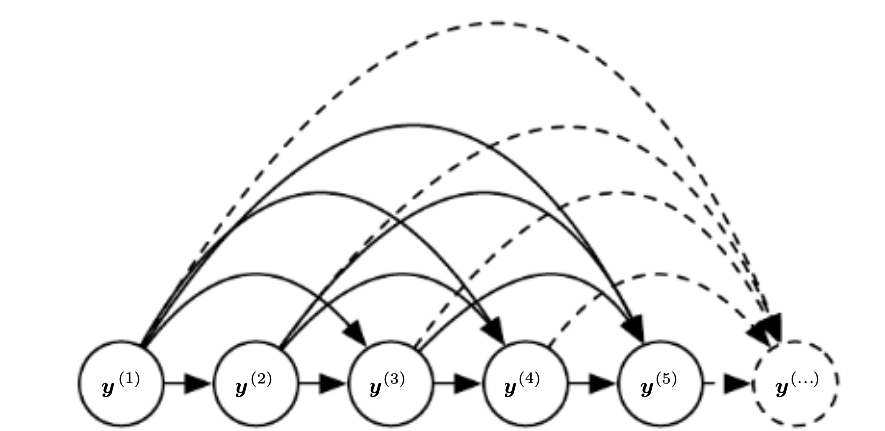
\includegraphics[height=4cm]{data/graph_model_1.png}
\end{frame}

\begin{frame}{Directed graphical models with RNN}
\begin{itemize}
\item RNN can represent the joint probability 
\item introduction of hidden units provides efficient parametrization
\item number of parameters is independent of sequence length
\item sparse representation, compared e.g. to table 
\end{itemize}
\vspace{1em}
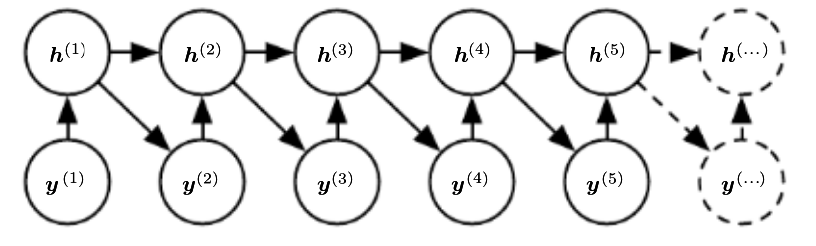
\includegraphics[height=2.5cm]{data/graph_model_2.png}
\end{frame}

\begin{frame}[beamer:0]{Notes}
\begin{itemize}
\item Direceted graphical models represent random variables and their influences/independence, similar to Markov chains (or Markov Random Fields).
\item A RNN can be used to give an efficient parametrization of these.
\item No input is used in this case, the hidden neurons $h^{(t)}$ are random variables which are deterministic given the values of their parents. 
\end{itemize}
\end{frame}

\begin{frame}{Bidirectional RNNs}
\centering
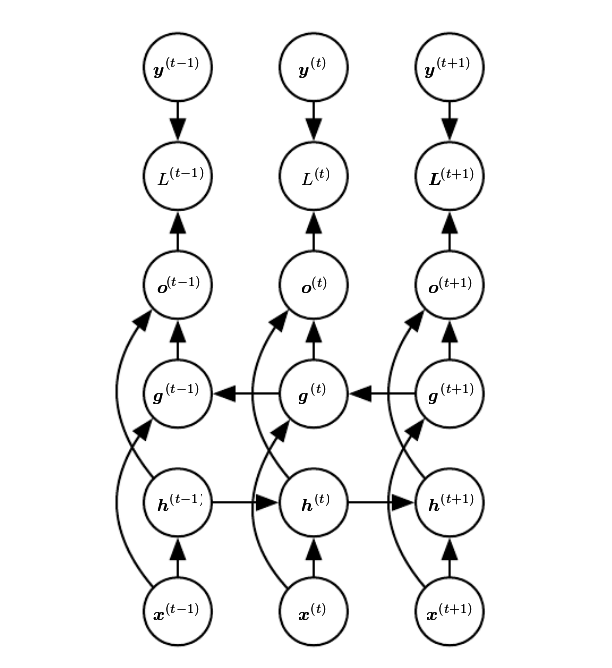
\includegraphics[height=8cm]{data/bidirectional.png}
\end{frame}

\begin{frame}[beamer:0]{Notes}
\begin{itemize}
\item In many applications an output depends not only on earlier but also on later inputs. E.g. in speech recognition the interpretation of the current sound may depend on sounds before and after this. 
\item The example architecture shows a RNN whose outputs depend on prior and later inputs. 
\item Such RNNs have similarities to convolutional neural networks, only that here a ``window'' of flexible rather than fixed size appears around a time step.
\item Forward and back-propagation can be performed as usual, only for the parameters associated with $g^{(t)}$  the gradient computation must start from the first time step rather than the last one.
\end{itemize}
\end{frame}

\begin{frame}{Encoder-Decoder Architectures}
\centering
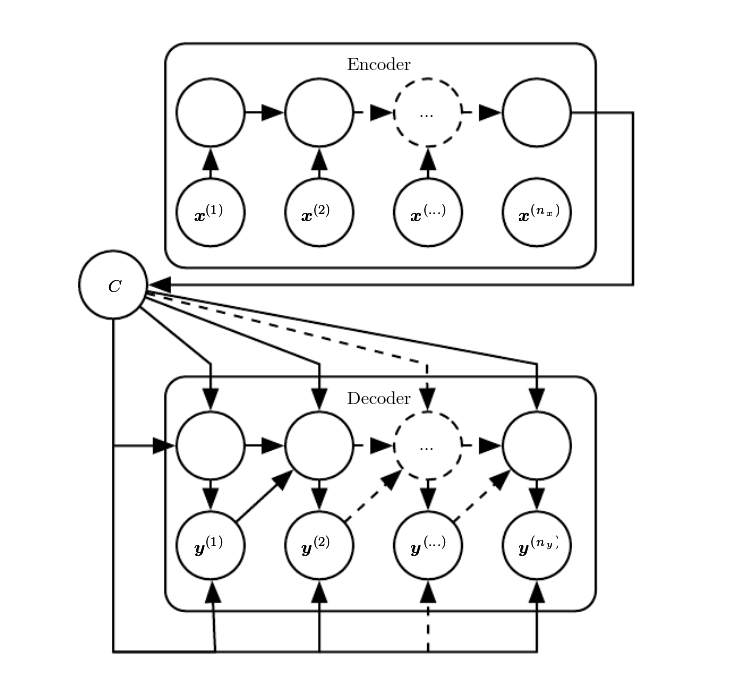
\includegraphics[height=8cm]{data/encode-decode.png}
\end{frame}

\begin{frame}[beamer:0]{Notes}
\begin{itemize}
\item Encoder-Decoder architectures allow to produce an output sequence whose length is independent of the length of the input sequence. Machine translation is a taks which requires this setting.
\item The vector $c$ contains all the information of the input sequence. This requires a high-dimension or input information may be lost. Some authors propose to use a variable length sequence at this point instead.
\end{itemize}
\end{frame}


\begin{frame}{Deep Recurrent Networks}
\centering
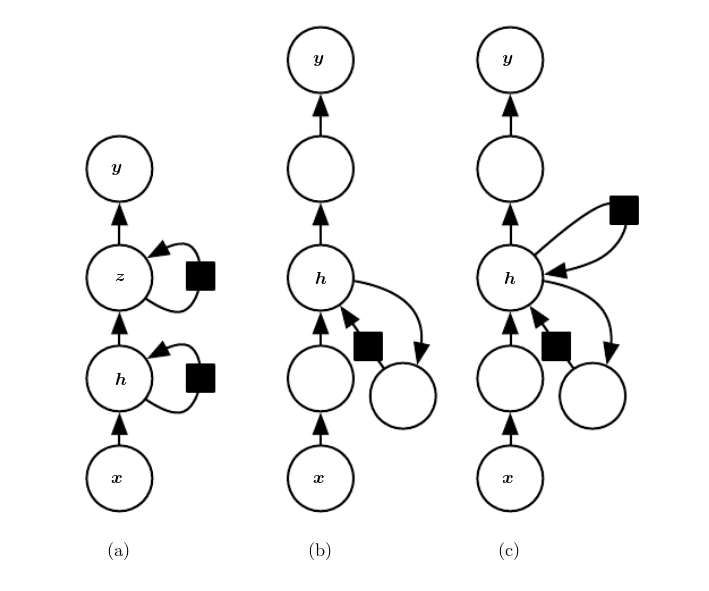
\includegraphics[height=8cm]{data/deep-rnn.png}
\end{frame}

\begin{frame}[beamer:0]{Notes}
\begin{itemize}
\item Black boxes in the figure symbolize that the information is passed forward/backward in the next time step.
\item Various configurations of recurrent layers are possible. Skip connections as in $(c)$ may be introduced to shorten the paths for the gradient backward pass, which can help to facilitate the training of the RNN.
\end{itemize}
\end{frame}

\begin{frame}{Recursive Neural Networks}
\centering
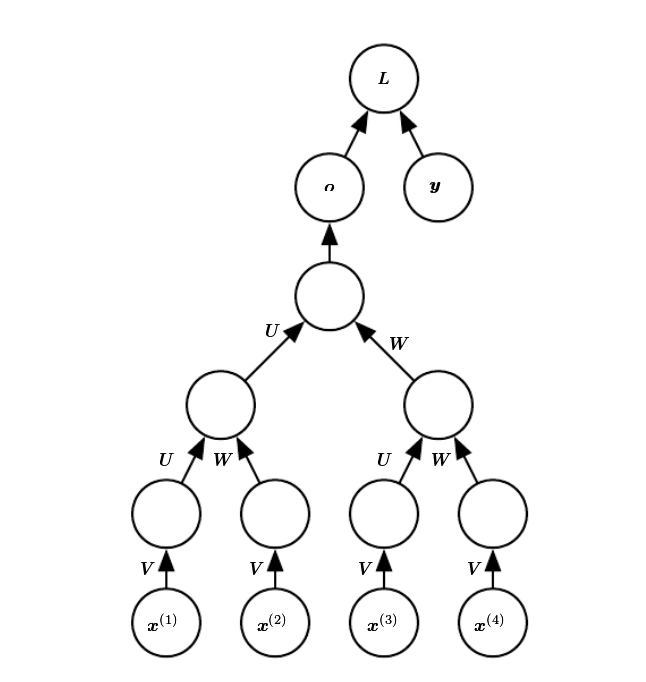
\includegraphics[height=8cm]{data/recursive.png}
\end{frame}

\begin{frame}[beamer:0]{Notes}
\begin{itemize}
\item RNN can also be generalized into recursive neural networks. The structure can then have the form of a tree which gives various possibilities to process the input information of variable length.
\end{itemize}
\end{frame}

\section{Long Term Dependencies}
\begin{frame}
\sectionpage
\end{frame}

\begin{frame}{Problem of Long Term Dependencies}
\begin{itemize}
\item in RNN's gradients are propagated over many stages, which can lead to vanishing or exploding gradients
\item the influence of an output vanishes over time 
\item challenge: How can we make information flow over long distances?
\end{itemize}
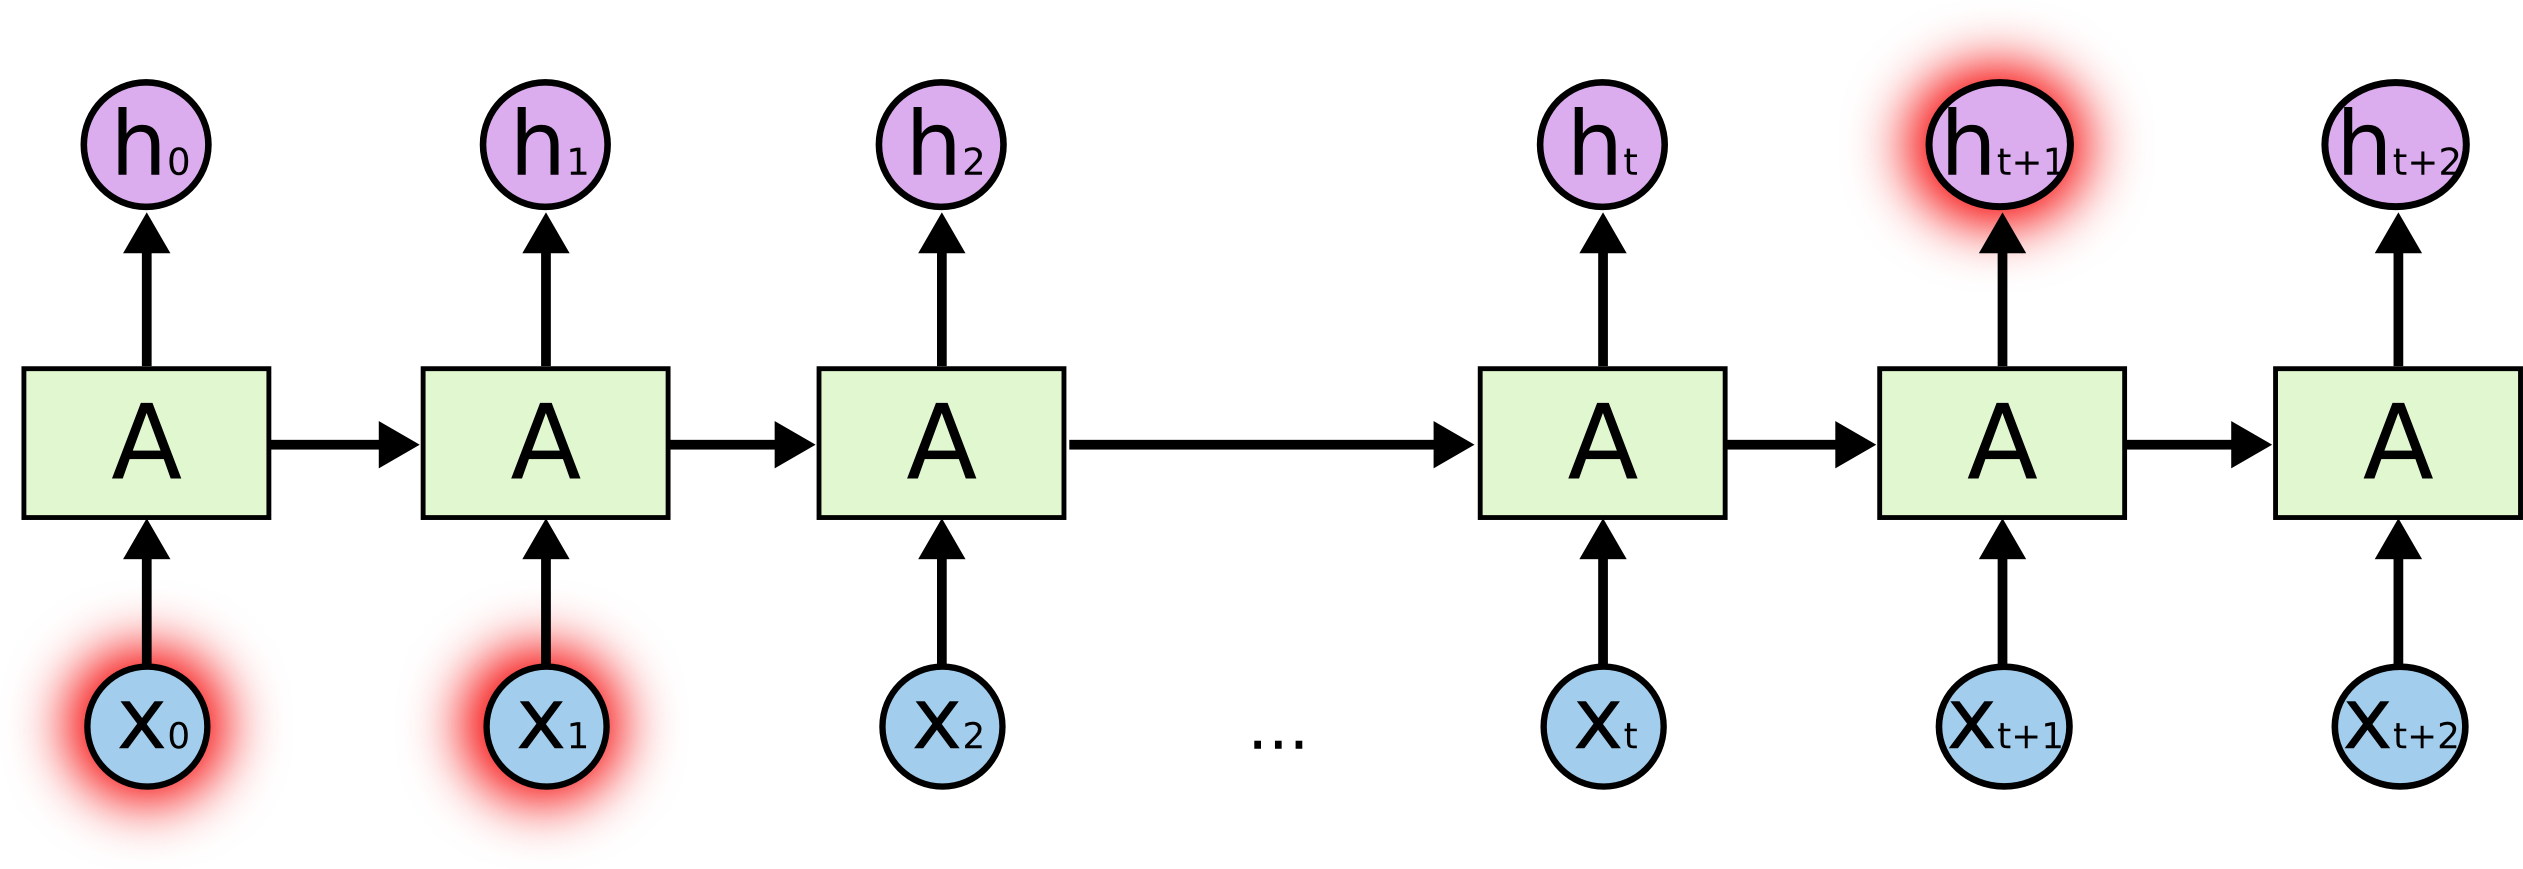
\includegraphics[height=2.5cm]{data/RNN-longtermdependencies.png}
\end{frame}

\begin{frame}{Techniques for Long Term Dependencies}
\begin{itemize}
\item Echo state networks
\item Gated RNN's - LSTM
\end{itemize}
\end{frame}

\begin{frame}{LSTM - Long Term Short Memory}
Idea: 
\begin{itemize}
\item have one state that flows over time and can be manipulated
\item gates control the information that is passed to the state
\item units are not connected through fixed weights but with dynamical connections
\end{itemize}
\end{frame}

\begin{frame}{Difference between normal RNN and LSTM}
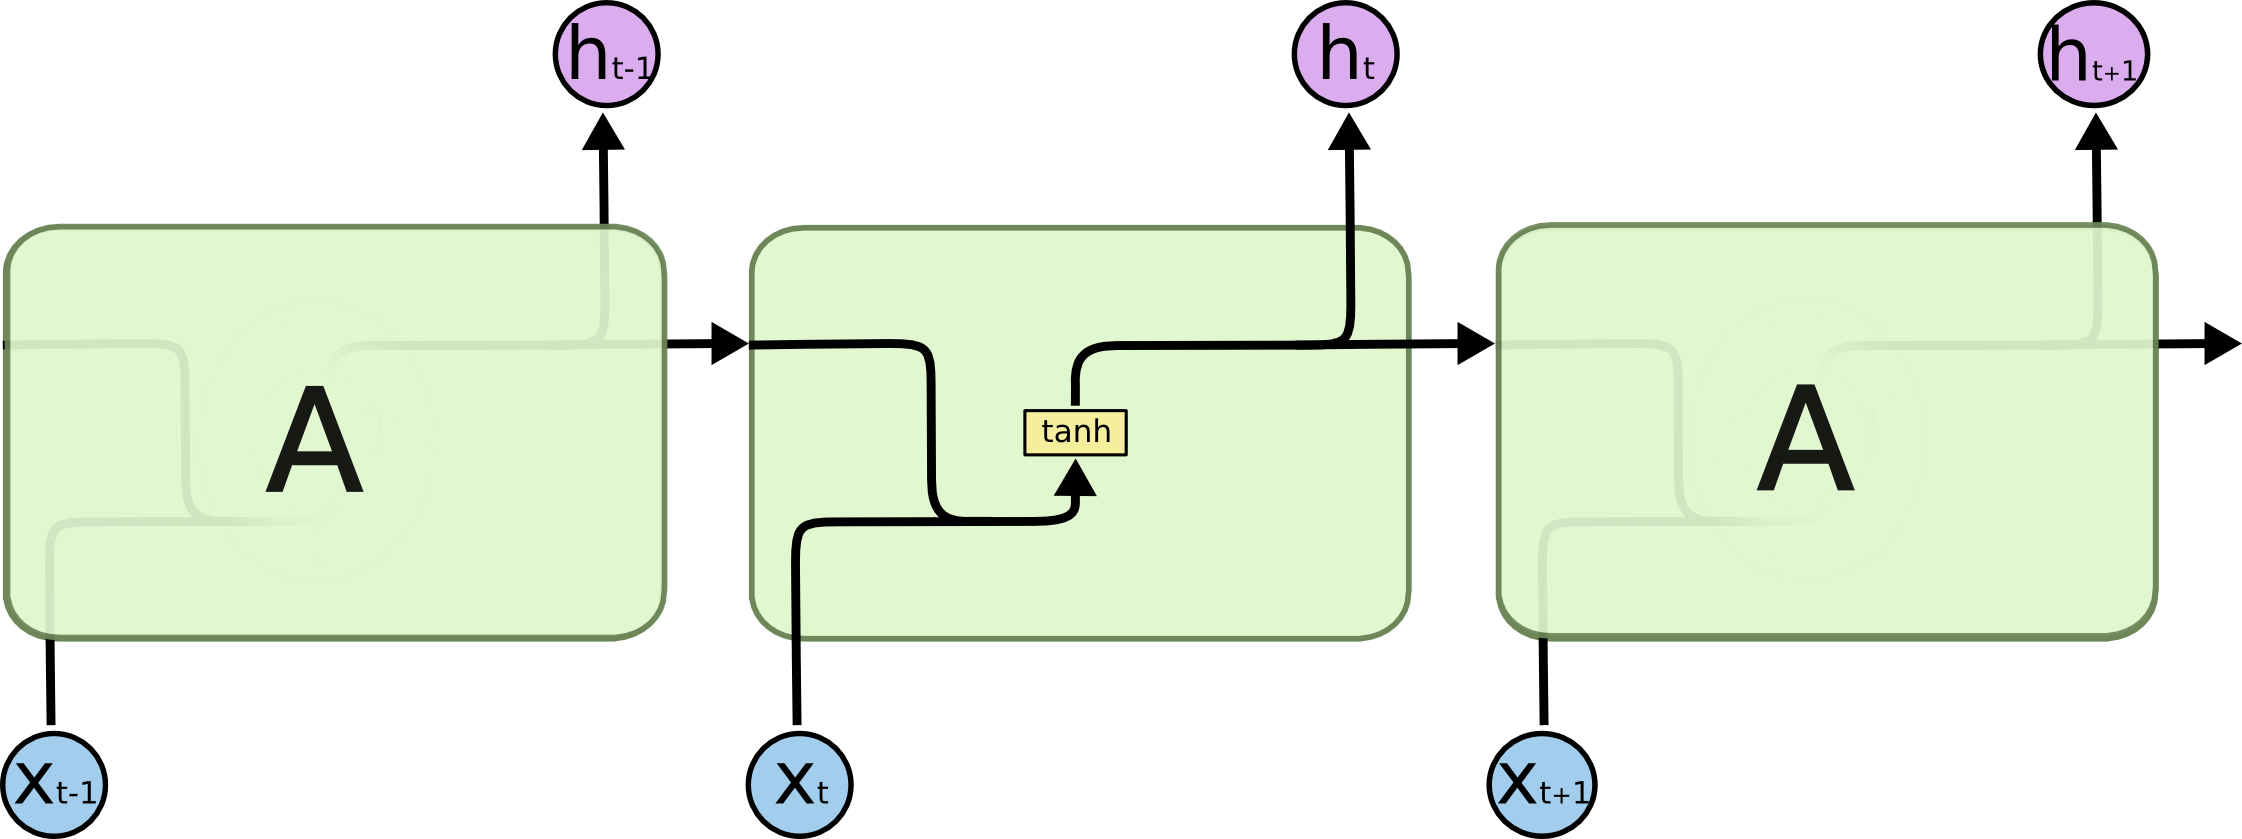
\includegraphics[height=3.0cm]{data/LSTM3-SimpleRNN.png}\\ 
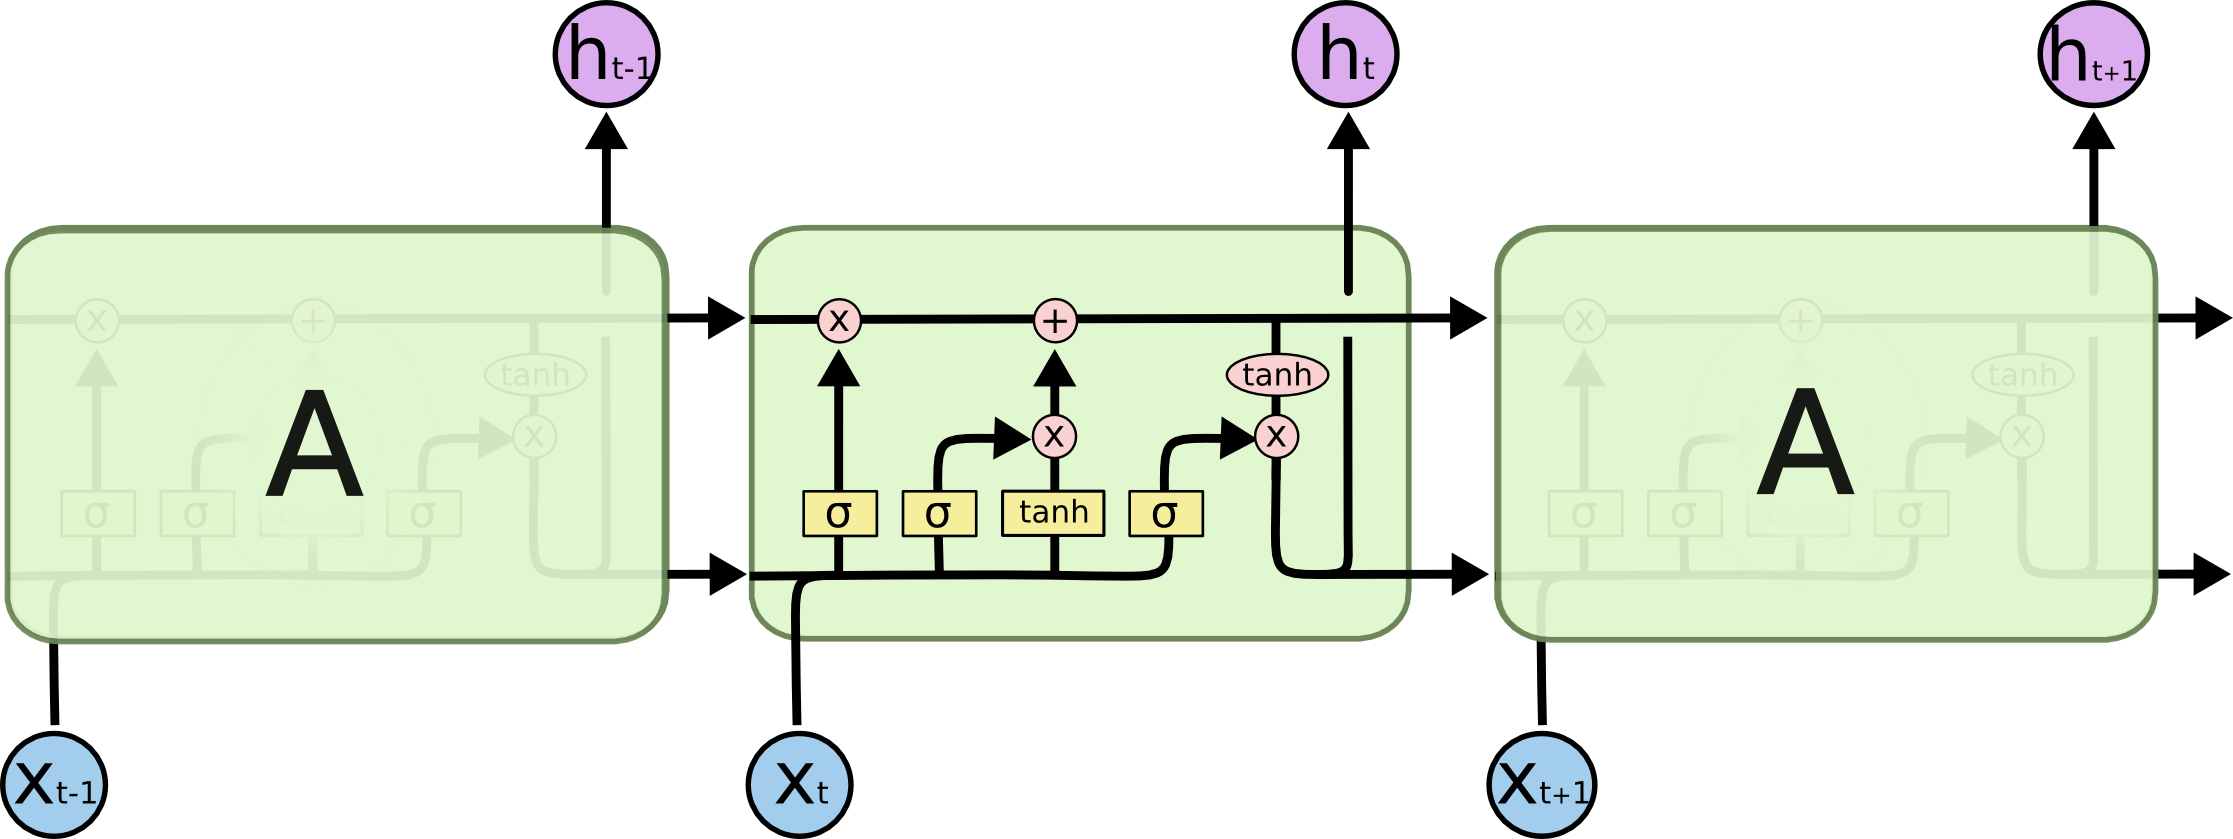
\includegraphics[height=3.0cm]{data/LSTM3-chain.png}\\
Source: (Great Blog!) http://colah.github.io/posts/2015-08-Understanding-LSTMs/ 
\end{frame}

\only<4|handout:1>{
There are 3 gates at a standard LSTM:\\
\begin{itemize}
\item Forget-Gate: gate that can delete information of the state
\item Input-Gate: decides, which values of the state are going to be updated with which information
\item Output-Gate: creates output from the state and the input
\end{itemize}
}

\begin{frame}{The Forget-Gate}
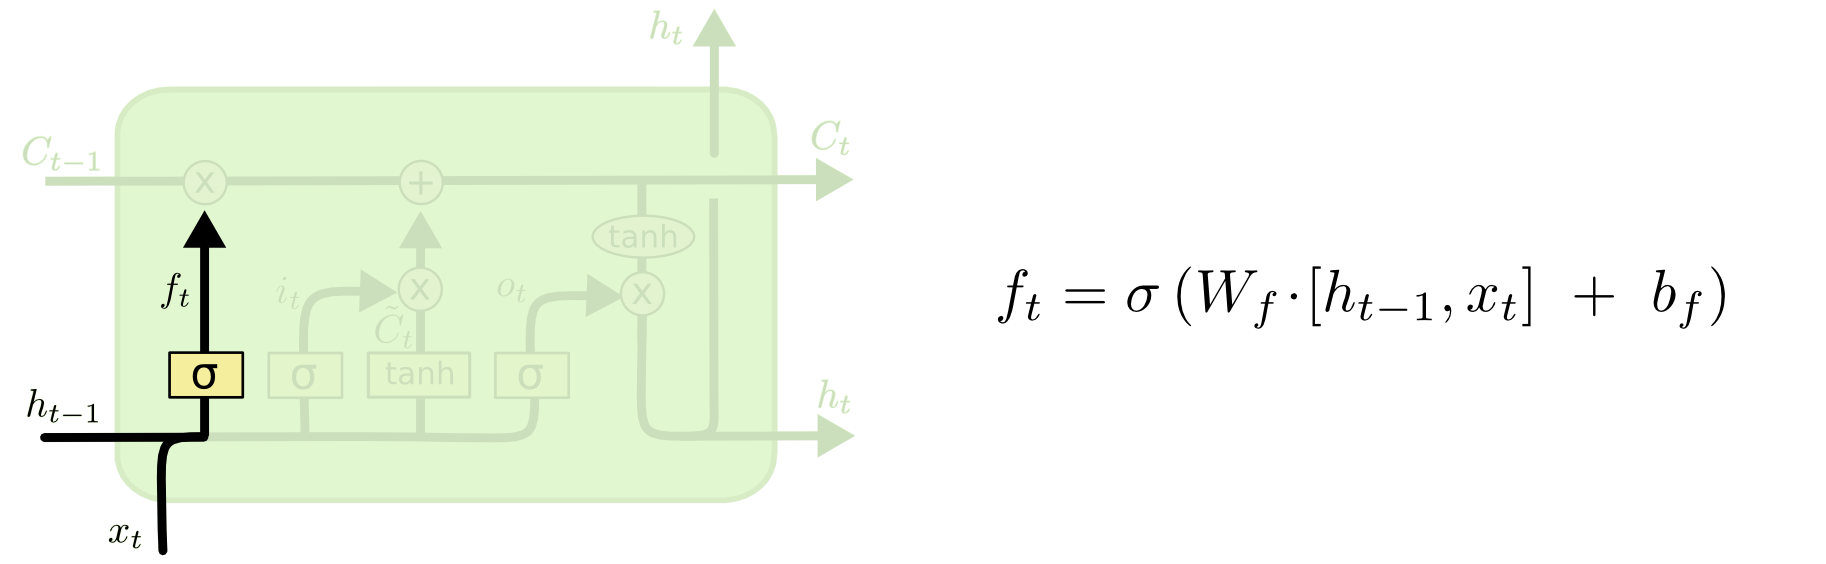
\includegraphics[height=3.0cm]{data/LSTM3-focus-f.png}\\ 
\end{frame}

\begin{frame}{The Input-Gate}
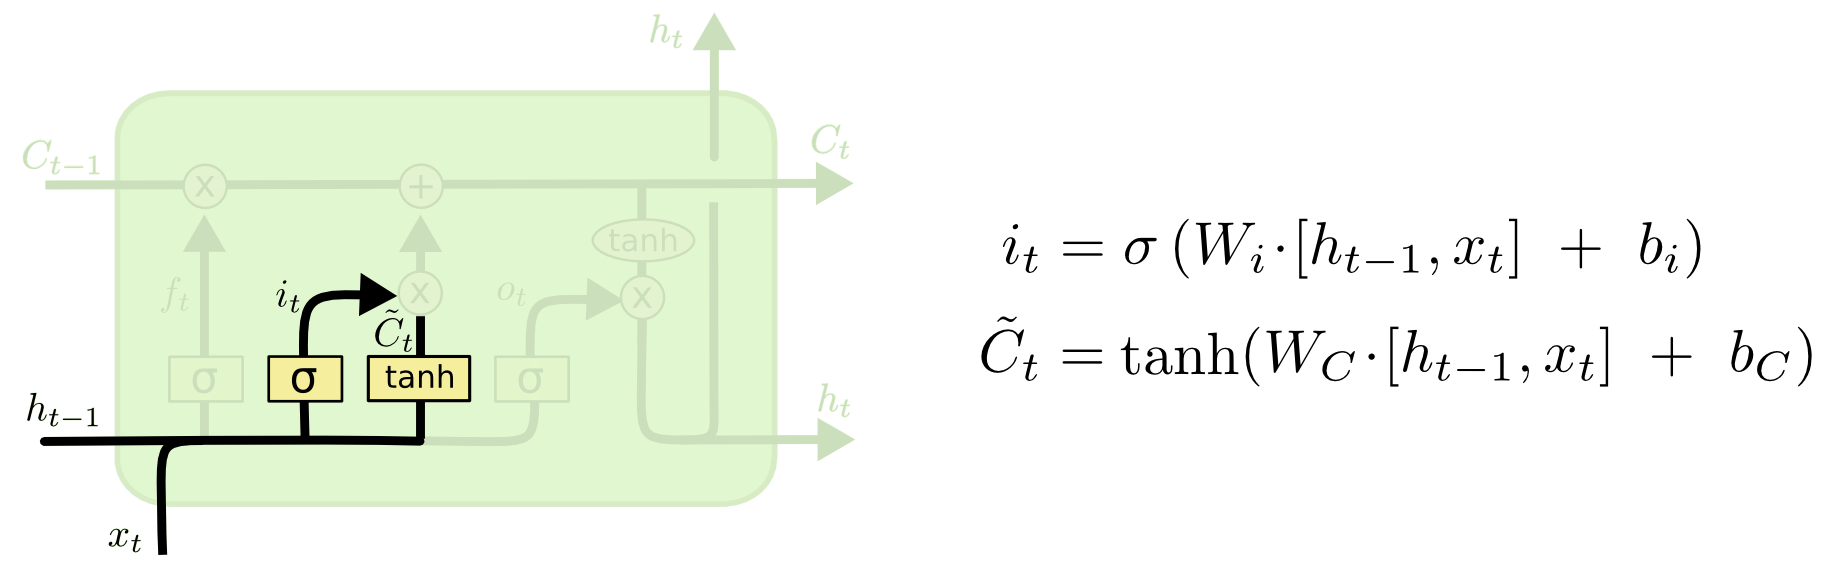
\includegraphics[height=3.0cm]{data/LSTM3-focus-i.png}\\ 
\end{frame}

\begin{frame}{The State-Update}
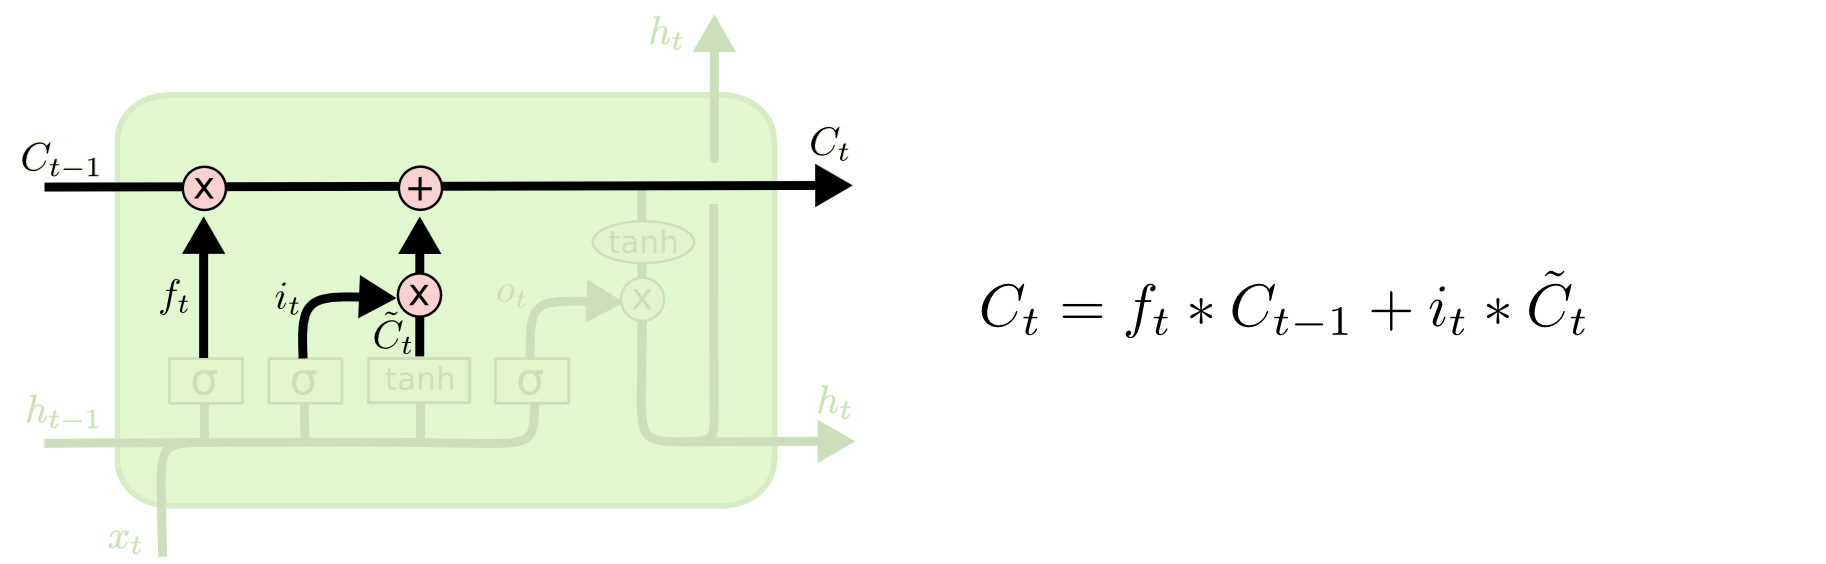
\includegraphics[height=3.0cm]{data/LSTM3-focus-C.png}\\ 
\end{frame}

\begin{frame}{The Output-Gate}
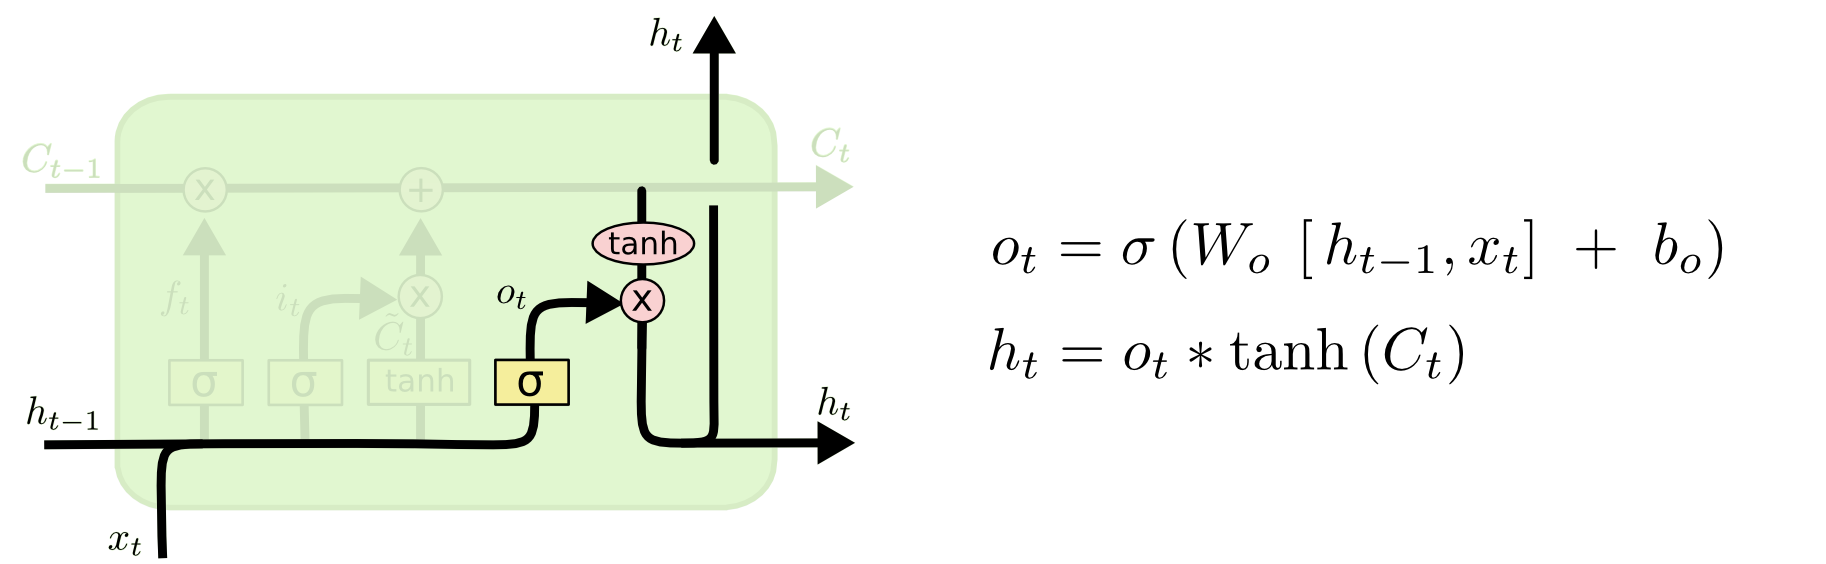
\includegraphics[height=3.0cm]{data/LSTM3-focus-o.png}\\ 
\end{frame}

\section{Programming Project}
\begin{frame}
\sectionpage
\end{frame}

\begin{frame}{The Real World Problem}
Semantic Segmentation\\
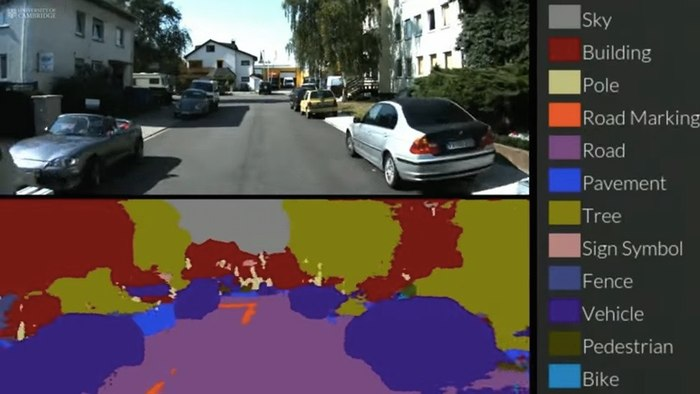
\includegraphics[height=5.0cm]{data/segnet.jpg}\\ 
Source: University of Cambridge\\
\only<5|handout:1>{
Each pixel from a camera image should be annotated with a class ("tree","car","street",..). This technique is neccessary if it is not only important WHAT objects you can see in an image but also WHERE they are, for example in the case of autonomous cars.
}
\end{frame}

\begin{frame}{My Toy-Example}

\includegraphics[height=3.0cm]{data/greyimage.jpg} \t Greyscale Image\\ 

\includegraphics[height=3.0cm]{data/segmentation.jpg} \t Segmentation: Road- Not Road\\ 
\end{frame}

\begin{frame}{The robot car}
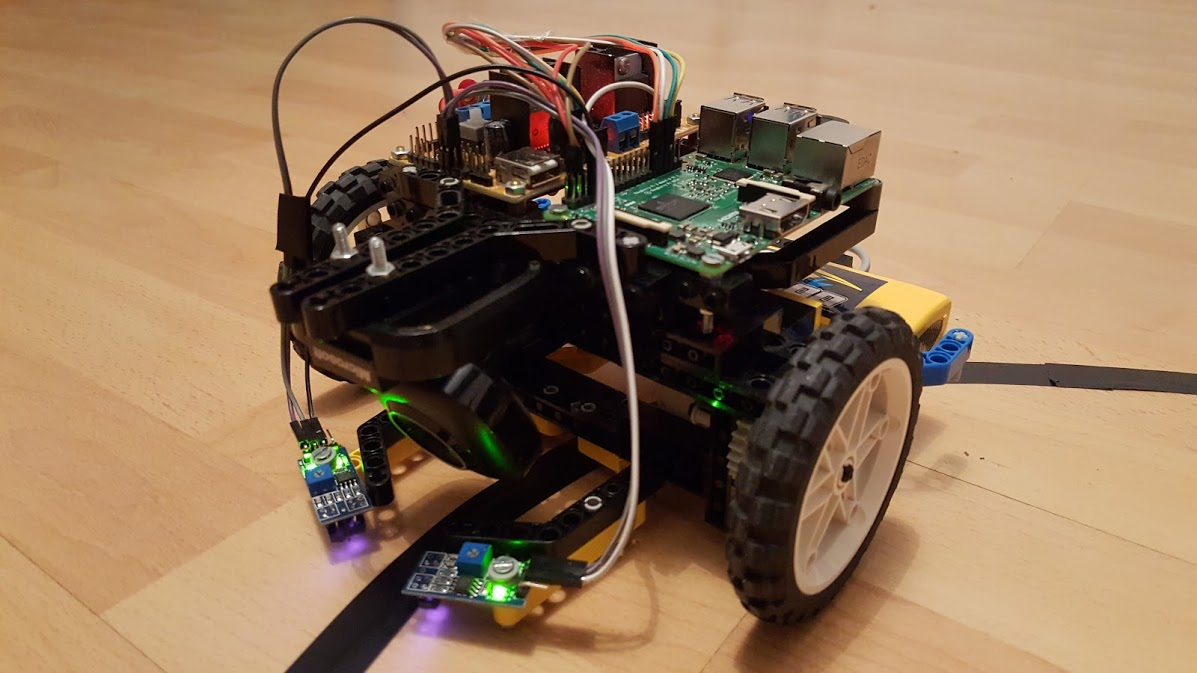
\includegraphics[height=6.0cm]{data/robot.jpg}\\ 
Light-sensors to follow the black line, webcam to take pictures.
\end{frame}

\begin{frame}{Idea}
\begin{tikzpicture}[->, scale=0.6]
\tikzset{VertexStyle/.style = {shape=rectangle, inner sep = 2pt, minimum size = 24pt, draw, font=\tiny}}
\tikzset{EdgeStyle/.style = {->, thick}}
  	\SetGraphUnit{1}
 	
  	\Vertex[x=10, y=0, L={
\includegraphics[height=1.5cm]{data/greyimage.jpg}}]{x3}
	\Vertex[x=10, y=3, L={Conv. Net}]{h3}
	\Vertex[x=10, y=6, L={
\includegraphics[height=1.5cm]{data/segmentation.jpg}}]{o3}  	
  	\Edge[](x3)(h3)
  	\Edge[](h3)(o3)
  	
  	\Vertex[x=15, y=0, L={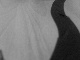
\includegraphics[height=1.5cm]{data/greyimage2.jpg}}]{x4}
	\Vertex[x=15, y=3, L={Conv. Net}]{h4}
	\Vertex[x=15, y=6, L={
\includegraphics[height=1.5cm]{data/segmentation2.jpg}}]{o4}
  	
  	\Edge[](x4)(h4)
  	\Edge[](h4)(o4)
  	\Edge[](o3)(h4)
  	
  	  	\Vertex[x=20, y=0, L={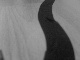
\includegraphics[height=1.5cm]{data/greyimage3.jpg}}]{x5}
	\Vertex[x=20, y=3, L={Conv. Net}]{h5}
	\Vertex[x=20, y=6, L={
\includegraphics[height=1.5cm]{data/segmentation3.jpg}}]{o5}
  	
  	\Edge[](x5)(h5)
  	\Edge[](h5)(o5)
  	\Edge[](o4)(h5)
\end{tikzpicture}
\only<5|handout:2>{
The aim is to construct an RNN which obtains the previous segmentation and moving direction as well as the actual image as an input. This network is than able to interpret an image in the context of a sequence of images.
}
\end{frame}

\begin{frame}{Challenges}
\begin{itemize}
\item get a lot of training data
\item generate the ground trouth automatically
\item make the task neither too complicated nor too easy
\end{itemize}
\end{frame}

\begin{frame}{Generation of data and ground truth}
\begin{tikzpicture}[->, scale=0.6]
\tikzset{VertexStyle/.style = {shape=rectangle, inner sep = 2pt, minimum size = 24pt, draw, font=\tiny}}
\tikzset{EdgeStyle/.style = {->, thick}}
  	\SetGraphUnit{1}
 	
  	\Vertex[x=5, y=9, L={
\includegraphics[height=1.5cm]{data/47g.jpg} 
\includegraphics[height=1.5cm]{data/48g.jpg} 
\includegraphics[height=1.5cm]{data/49g.jpg}}]{g}

  	\Vertex[x=0, y=4, L={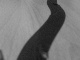
\includegraphics[height=1.0cm]{data/47gd.jpg} 
\includegraphics[height=1.0cm]{data/48gd.jpg} 
\includegraphics[height=1.0cm]{data/49gd.jpg}}]{gd}

  	\Vertex[x=10, y=2, L={
\includegraphics[height=1.0cm]{data/47s.jpg} 
\includegraphics[height=1.0cm]{data/48s.jpg} 
\includegraphics[height=1.0cm]{data/49s.jpg}}]{s}
  	
  	\Edge[label=Add Random Constant](g)(gd)
  	\Edge[label=Pixelwise Threshold](g)(s)
  	
  	  	\Vertex[x=20, y=0, L={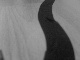
\includegraphics[height=1.5cm]{data/greyimage3.jpg}}]{x5}
	\Vertex[x=20, y=3, L={Conv. Net}]{h5}
	\Vertex[x=20, y=6, L={
\includegraphics[height=1.5cm]{data/segmentation3.jpg}}]{o5}
  	
  	\Edge[](x5)(h5)
  	\Edge[](h5)(o5)
  	\Edge[](o4)(h5)
\end{tikzpicture}

\only<5|handout:3>{
From greyscale images the trainingset was generated:
\begin{itemize}
\item the input images are the pictures distorted with a random constant value
\item the ground truth ("labels") are generated with a simple threshold in the black value
\end{itemize}

Why so complicated?\\
The ground truth needs to be generated automatically, because it is not possible to obatain enough training data when the data is labled by hand.\\
Still the network should learn more than a simple threshold (too easy!).
}
\end{frame}

\begin{frame}{Architecture of the RNN}
\begin{tikzpicture}[->, scale=0.6]
\tikzset{VertexStyle/.style = {shape=rectangle, inner sep = 2pt, minimum size = 24pt, draw, font=\tiny}}
\tikzset{EdgeStyle/.style = {->, thick}}
  	\SetGraphUnit{1}
 	
  	\Vertex[x=0, y=1, L={
\includegraphics[height=1.0cm]{data/47s.jpg}}]{s}
  	\Vertex[x=3, y=1, L={direction}]{d}
  	\Vertex[x=9, y=1, L={
\includegraphics[height=1.0cm]{data/48g.jpg}}]{g}
  	
  	\Vertex[x=1, y=3, L={Conv. Layer, 5 filters, stride 5x5}]{L1}
  	\Vertex[x=9, y=3, L={Conv. Layer, 5 filters, stride 5x5}]{L2}
  	
  	\Vertex[x=5, y=5, L={Conv. Layer, 5 filters, stride 5x5}]{L3}
  	\Vertex[x=5, y=7, L={Conv. Layer, 3 filters, stride 5x5}]{L4}
  	\Vertex[x=5, y=9, L={Conv. Layer, 1 filter, stride 1x1}]{L5}
  	\Vertex[x=5, y=11, L={
\includegraphics[height=1.0cm]{data/48s.jpg}}]{o}
  	
  	\Edge[](s)(L1)
  	\Edge[](d)(L1)
  	\Edge[](g)(L2)
  	\Edge[](L1)(L3)
  	\Edge[](L2)(L3)
  	\Edge[](L3)(L4)
  	\Edge[](L4)(L5)
  	\Edge[](L5)(o)
  	
\end{tikzpicture}
\end{frame}

\begin{frame}{Programming: Tensorflow (ML-library for python)}
\begin{itemize}
\item really easy to use
\item computational efficient
\item builds 'graph' of the neural network which consists of optimized operations
\end{itemize}
\end{frame}

\begin{frame}{Code}
All available under: \url{https://github.com/arneschmidt/RNN_project/}\\ 
Feel free to change the RNN and try things out!
\only<5|handout:4>{
Ideas to try out:
\begin{itemize}
\item different architecture (change number of layers, stride, filters etc.)
\item use an LSTM for the prediction of the direction
\item use an LSTM for the segmentation
\end{itemize}
}
\end{frame}

\begin{frame}{First results}
Comparison of RNN with normal CNN:\\
Pixelwise accuracy:\\
Image only: 92.45 \\
Image+previous segmentation (RNN): 98.64 \\
(same architecture and 10.000 training steps)
\end{frame}

\begin{frame}{Training procedure}
1. 5000 iterations with teacher forcing, batches of 10 images\\
2. 5000 iterations with sequences of 5 images\\
3. 5000 iterations with sequences of 10 images\\
\end{frame}

\begin{frame}{After 0 iterations}
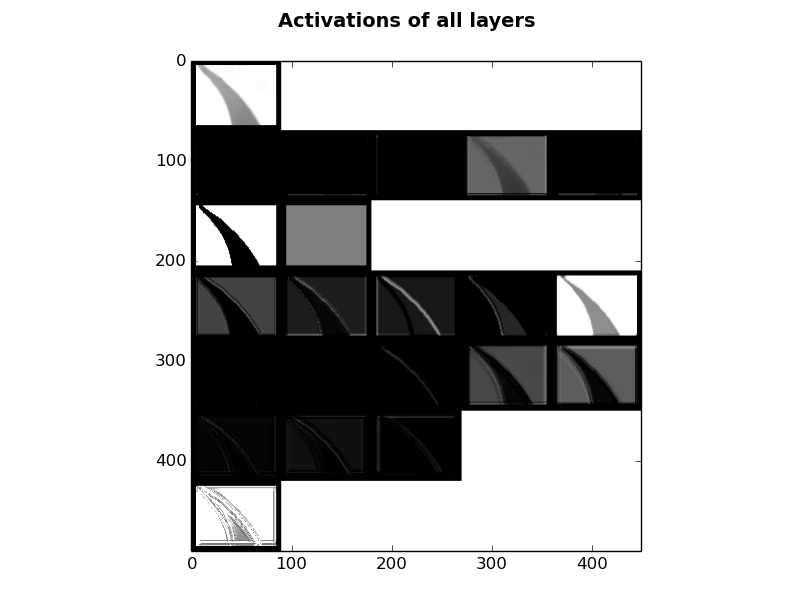
\includegraphics[height=8.0cm]{data/activations/output-0.png}\\ 
\end{frame}

\begin{frame}{After 100 iterations}
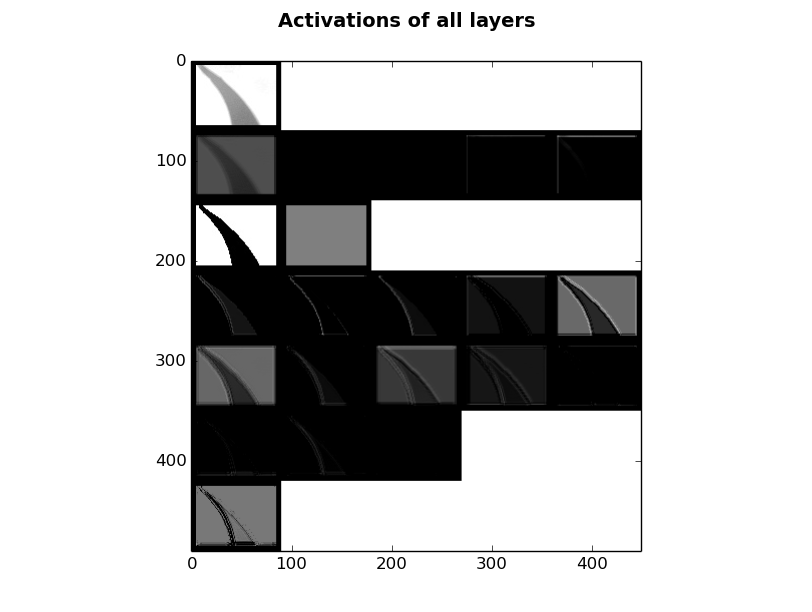
\includegraphics[height=8.0cm]{data/activations/output-100.png}\\ 
\end{frame}

\begin{frame}{After 200 iterations}
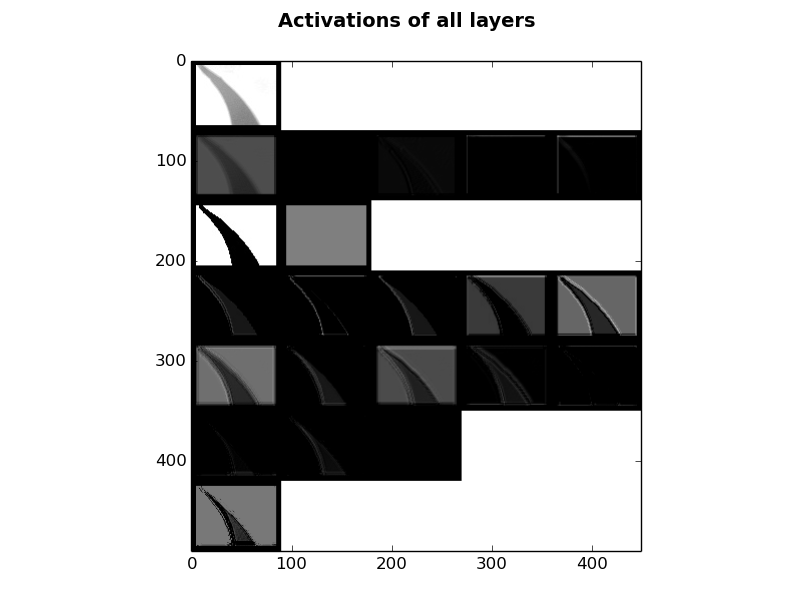
\includegraphics[height=8.0cm]{data/activations/output-200.png}\\ 
\end{frame}

\begin{frame}{After 300 iterations}
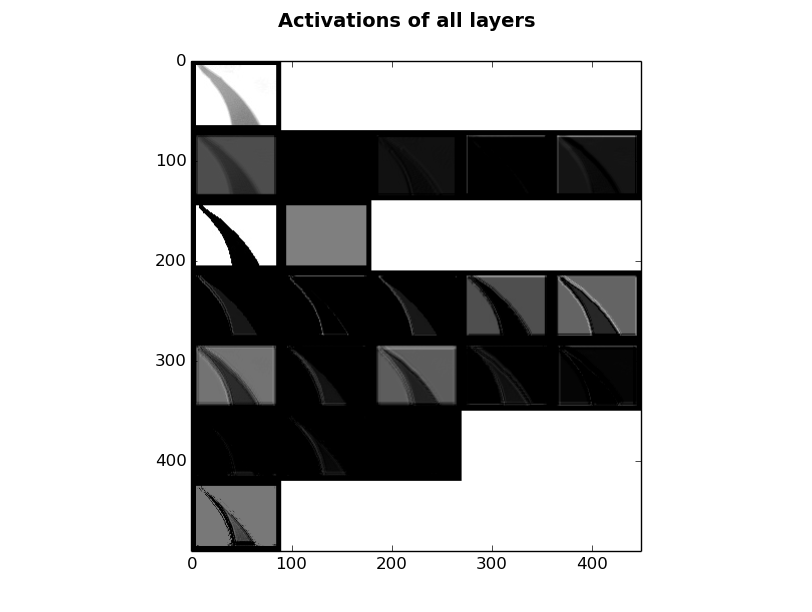
\includegraphics[height=8.0cm]{data/activations/output-300.png}\\ 
\end{frame}

\begin{frame}{After 400 iterations}
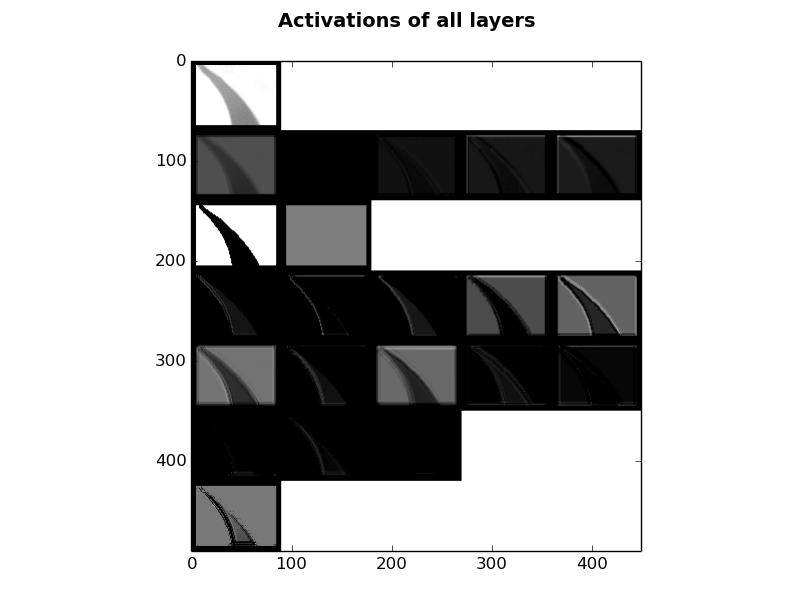
\includegraphics[height=8.0cm]{data/activations/output-400.png}\\ 
\end{frame}

\begin{frame}{After 500 iterations}
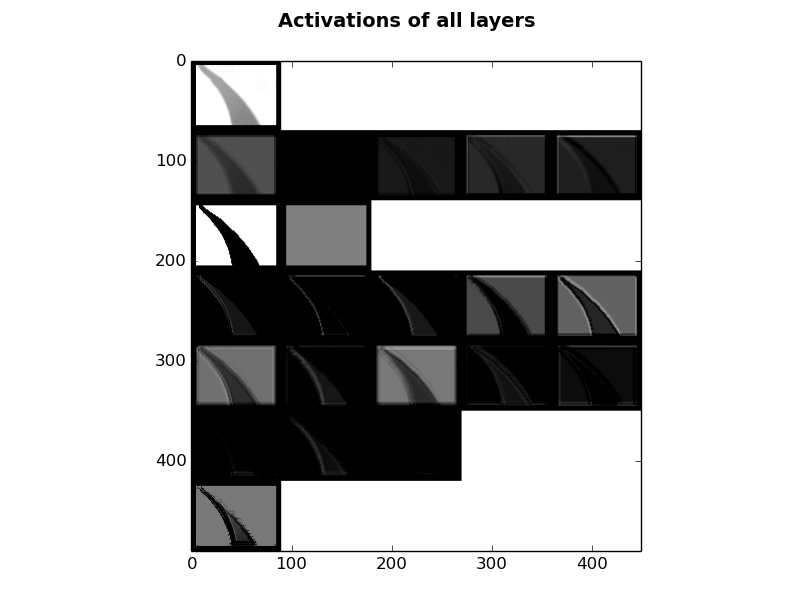
\includegraphics[height=8.0cm]{data/activations/output-500.png}\\ 
\end{frame}

\begin{frame}{After 600 iterations}
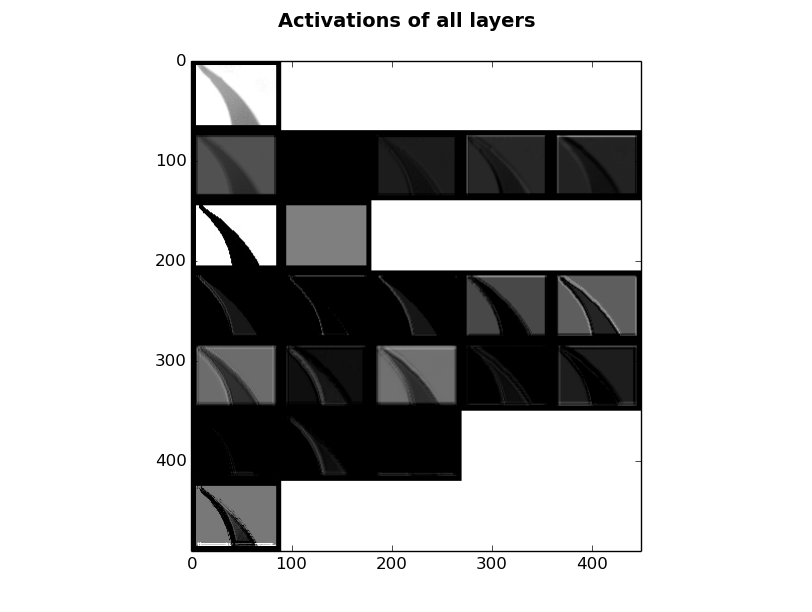
\includegraphics[height=8.0cm]{data/activations/output-600.png}\\ 
\end{frame}

\begin{frame}{After 700 iterations}
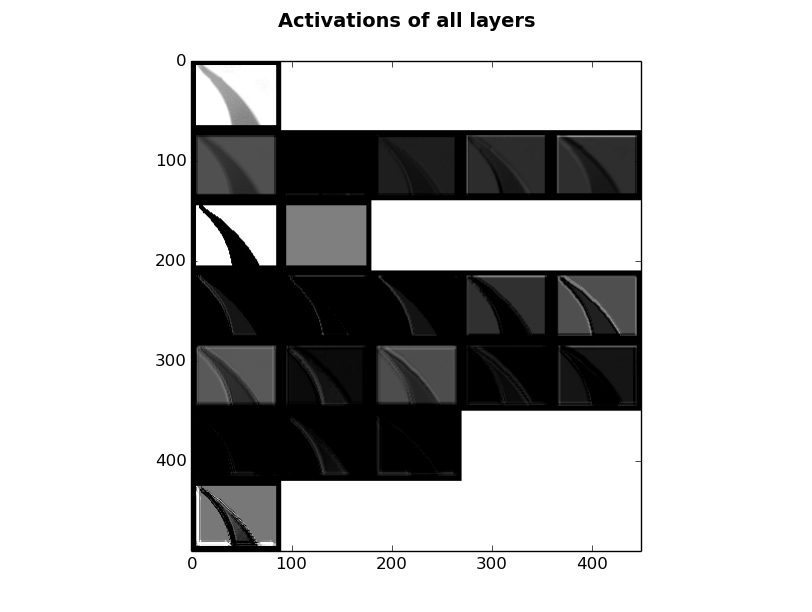
\includegraphics[height=8.0cm]{data/activations/output-700.png}\\ 
\end{frame}

\begin{frame}{After 800 iterations}
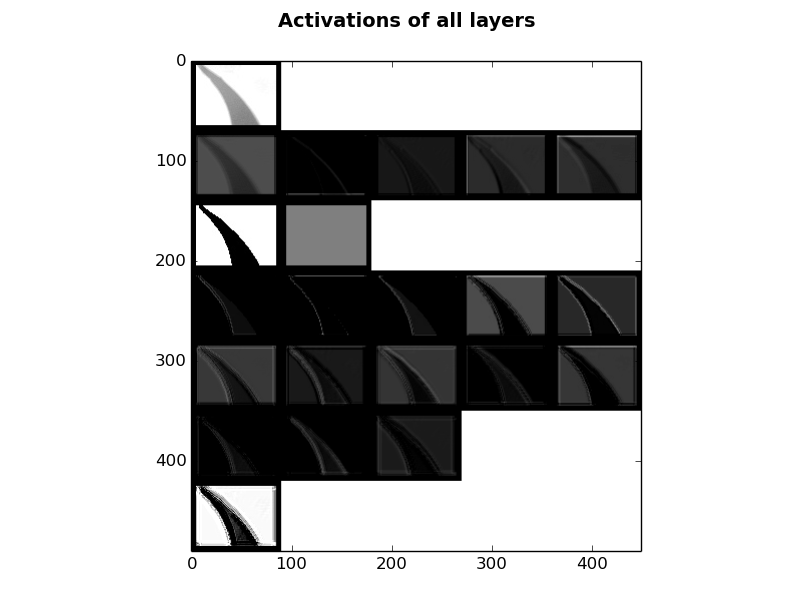
\includegraphics[height=8.0cm]{data/activations/output-800.png}\\ 
\end{frame}

\begin{frame}{After 900 iterations}
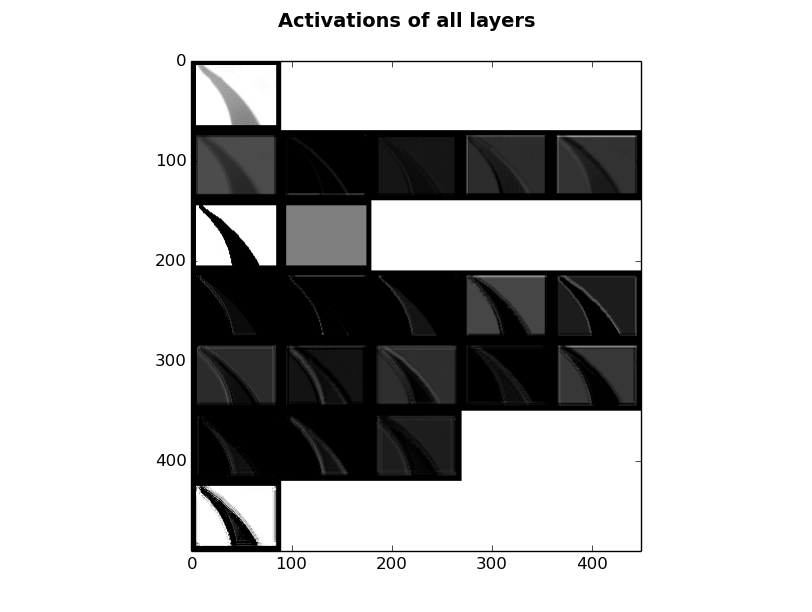
\includegraphics[height=8.0cm]{data/activations/output-900.png}\\ 
\end{frame}

\begin{frame}{After 1000 iterations}
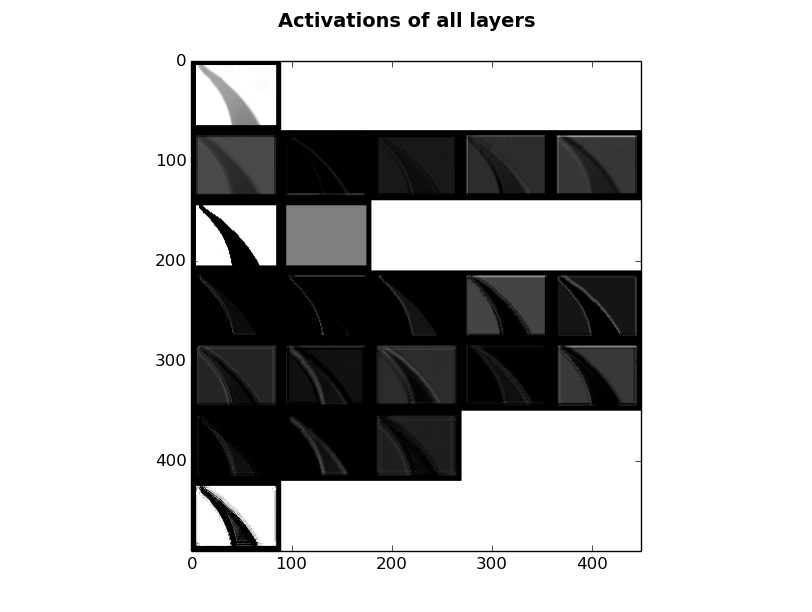
\includegraphics[height=8.0cm]{data/activations/output-1000.png}\\ 
\end{frame}

\begin{frame}{After 2000 iterations}
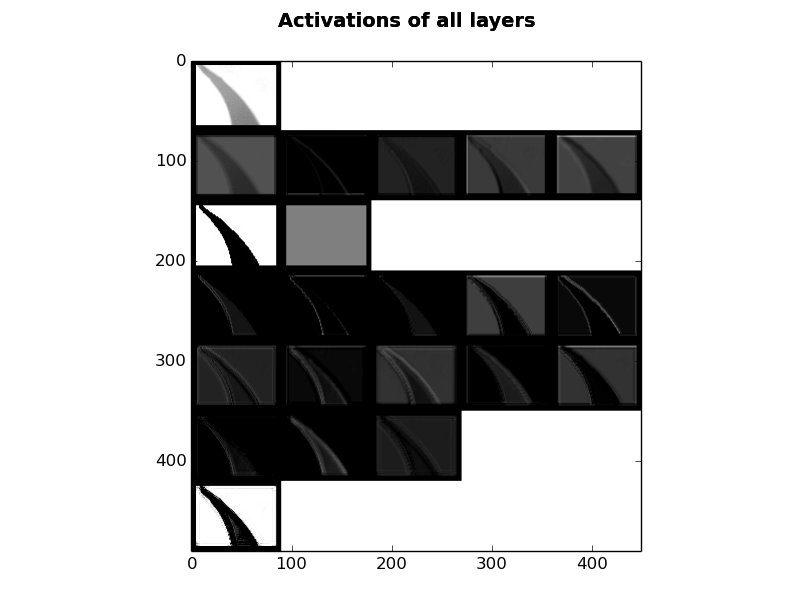
\includegraphics[height=8.0cm]{data/activations/output-2000.png}\\ 
\end{frame}

\begin{frame}{After 3000 iterations}
\includegraphics[height=8.0cm]{data/activations/output-3000.png}\\ 
\end{frame}

\begin{frame}{After 4000 iterations}
\includegraphics[height=8.0cm]{data/activations/output-4000.png}\\ 
\end{frame}

\begin{frame}{After 5000 iterations}
\includegraphics[height=8.0cm]{data/activations/output-5000.png}\\ 
\end{frame}

\begin{frame}{After 10000 iterations}
\includegraphics[height=8.0cm]{data/activations/output-10000.png}\\ 
\end{frame}

\begin{frame}{After 15000 iterations}
\includegraphics[height=8.0cm]{data/activations/output-15000.png}\\ 
\end{frame}

\section*{Final Remarks}
\begin{frame}{References}
\nocite{GoBeCo16}
\bibliographystyle{plain}
\tiny
\bibliography{data/literature}
\end{frame}

\end{document}
